%==========================================================%
% author: Simon Roth - www.systats.com 
%       Universität Stuttgart  
%       creation date: 24.02.2017, version: 0.1       
%       last update: - 30.3.2017
%==========================================================%

%%% Configurations ---
\documentclass{systats}


%%% Layout configurations
%\usepackage[top=2.5cm
%		, bottom=2cm
%		, left=2.5cm
%		, right=4cm]{geometry}

\usepackage[top=2.5cm,
 bottom=2cm,
 outer=4cm,
 inner=2.5cm, 
 heightrounded, 
 marginparwidth=3cm, 
 marginparsep = .5cm]{geometry}

\usepackage{csquotes}
\usepackage{lmodern}
\usepackage{multirow}
\usepackage{booktabs}
\usepackage[flushleft]{threeparttable}
%\usepackage{array}
\usepackage{caption}
%\usepackage{float}% If comment this, figure moves to Page 2
%\usepackage{flafter}
\usepackage[normalem]{ulem}
\usepackage{adjustbox}
\usepackage{mathtools}
\usepackage{fancyhdr}
\usepackage{amsmath}
\usepackage{pdflscape}
\usepackage{graphicx}
\usepackage{threeparttable}
\usepackage{ragged2e}
\usepackage{caption}
\usepackage{wrapfig}
\usepackage{lipsum}
\usepackage{floatflt}
\usepackage{pdflscape}
\usepackage{afterpage}
\usepackage{multicol}
\usepackage{capt-of}% or use the larger `caption` package
\usepackage{tabularx}
\usepackage{placeins}


\usepackage{lscape}
\usepackage{rotating}
\usepackage{epstopdf}
%\restylefloat{figure}
%%% language control, order matters
% [english, ngerman] = German
% [ngerman, english] = English
\usepackage[ngerman, english]{babel}
\usepackage{xcolor}

\usepackage{lmodern}


\makeatletter
\ifcase \@ptsize \relax% 10pt
\newcommand{\miniscule}{\@setfontsize\miniscule{4}{5}}% \tiny: 5/6
\or% 11pt
\newcommand{\miniscule}{\@setfontsize\miniscule{5}{6}}% \tiny: 6/7
\or% 12pt
\newcommand{\miniscule}{\@setfontsize\miniscule{5}{6}}% \tiny: 6/7
\fi
\makeatother
\usepackage[round]{natbib}

\setcitestyle{notesep={: }}
\setcitestyle{aysep={}} 

\usepackage{framed}
\newenvironment{quotationb}%
{\begin{leftbar}\begin{quotation}}%
{\end{quotation}\end{leftbar}}


\fancyhf{}
\renewcommand{\sectionmark}[1]{\markright{#1}}
%%% header
\fancyhead[RE,LO]{\fancyplain{}{\rightmark}} 
\rhead{\thepage}
\rfoot{\fancyplain{}{}}
\pagestyle{fancy}

%\rhead{\fancyplain{}{MyName}}
\newcommand{\ackname}{Acknowledgements}


%%% redefine \maketitle
\renewcommand{\maketitle}{
	\begin{titlepage}
		\begin{center}
			\setlength{\parskip}{0pt}
			
			%	    \begin{flushright}
			%	    \colorbox{darkgray}{\color{white}{\Large \textsf{\headerimg}}}
			%             \end{flushright}
			\begin{multicols}{2}
				\flushleft
				{Prof. Dr. Angelika Vetter\par}
				%{Seminar: Representative, direct and\\ cooperative participation in comparison\par}
				{Institute for Social Sciences\par}
				{Department of Political Systems \&\par}
				{Political Sociology}
				\begin{flushright}
					
\includegraphics[width=7cm]{images/logo_stuttgart.jpg}
				\end{flushright}
			\end{multicols}
			\vspace*{2mm}
			\center
			{\LARGE {Seminar Paper} \par}
			
			\vspace*{10mm}
			
			
			{\fontsize{26}{38} {\bfseries Direct Democracy in Europe} \par}
			\vspace*{1mm}
			{ \Large A Cross-National Examination of the Link Between Direct Democracy and Satisfaction with Democracy in 31 countries}
			\vspace*{10mm}
			
			\begin{multicols}{2}
				\center
				Author: Fabio Votta, B.A.\\
				Email: \href{mailto:fabio.vottagmail.com}{fabio.vottagmail.com}\\
				Student ID: 2891518\\
				
				Author: Rosa Seitz, B.A.\\
				Email: \href{mailto:rosa.marie.seitzgmail.com}{rosa.marie.seitzgmail.com}\\
				Student ID: 2876533\\
			\end{multicols}
			
			
			\vspace*{5mm}
			
			
			
			
			
			\vspace*{5mm}
			{Date of Submission: 30.03.2018 \par} %\date{xxx}
			
		\end{center}
		\vspace*{2mm}
		\begin{abstract}
			\justifying
			\noindent This seminar paper seeks to investigate deliberation and its relationship to regime support across the world. This is accomplished by exploring the relevant literature and deriving hypotheses from it, which are subsequently tested by using survey data covering 113 countries and 306,047 individual respondents. Given that self-reported regime support is expected to be biased, a weight is applied to account for possible distortions of the data, though results are also reported for the unweighted variable due to the experimental nature of this weight. As this paper is the first known to the authors that examines the effect of deliberation on regime support in a cross-country design, the used deliberation measurement, 
		\end{abstract}
		\vspace*{2mm}
		\center		
		{\large {Seminar: Representative, direct and cooperative participation in comparison} \par}
		
	\end{titlepage}
}


\begin{document}



%%% Title page
\maketitle

\clearpage


%%% toc
\newpage
\contents
\clearpage
\listoffigures
\clearpage
\listoftables

%++++++++++++++++++++++++++++++++++++++++++++++++++++++++++%
% Main Part
%++++++++++++++++++++++++++++++++++++++++++++++++++++++++++%
\clearpage
\setstretch{1.5}
\justify
%--------------------------------- Introduction ---------------------------------%
\section{Introduction} 

Direct democracy has been a topic of interest to political theory and empirical research for a long time. It is often asserted that direct democracy is closest to the ideal form of democracy, which is rule of the people and by the people themselves. In this light, direct democratic institutions are an often discussed remedy of the contemporary “crisis” of representative democracy which is postulated by some scholars \citep[cf.][]{pogrebischi2015}. Therefore, the causes and effects of direct democracy are of great interest to empirical research. For example, studies indicate positive effects on political efficacy \citep[cf.][]{bernhardbuehlmann2014} and satisfaction with democracy \citep[cf.][]{stadelmannvatter2012}. However, other authors have pointed out that direct democracy could exclude minorities and might foster inequalities in political participation \citep[cf.][]{merkelritzi2017}. Effects of direct democracy are sometimes heavily disputed, empirical research does not always provide conclusive evidence and many questions remain unanswered. In this context, quantitative comparative research has assigned great importance to the question of how to measure direct democracy, as empirical results rely heavily on the way direct democracy is operationalized. In the literature, different approaches to this question can be identified, having some elements in common but diverging in many ways. 

The aim of this work is to systematically compare selected approaches to the measurement of direct democracy on the national level in a theoretical and empirical way, as well as to examine data sources on direct democratic institutions in regard to their usability for quantitative research. It has to be noted, that this paper does not aim at giving a complete overview of the literature in terms of operationalization and measurement. Instead, only a few contemporary approaches are selected and addressed more thoroughly. In many studies, direct democracy is operationalized with a single dummy variable that specifies the existence of one specific institution (for example a citizens’ initiative dummy \citealp[as in][]{bernhardbuehlmann2014}). Such studies were not examined in this paper, as the focus here lies on measurements that account for the multidimensionality of direct democracy, which cannot be captured with a simple dummy variable. Furthermore, while the study of subnational direct democratic institutions is a worthwhile task, we primarily focus on national level measurements of direct democracy for the sake of a common thread across this work. The approaches examined theoretically and empirically are derived from different studies or datasets, namely: \citealp[][]{gherghina2016}, a subcomponent of the Democracy Barometer, \citealp[][]{peters2016}, \citealp[][]{fiorino2017}, and \citealp[][]{altman2017}/ \citealp[][]{coppedge2017data}.

The following Chapter \ref{challenges} discusses some of the general challenges in measuring direct democracy as well as criteria relevant to the measurement of direct democracy (like the decisiveness or ease of initiation/approval). In Chapter \ref{data}, some of the available data sources on direct democracy are briefly examined in regard to their content and scope, as well as their usability for quantitative research (the \textit{IDEA-Database}, the \textit{“Varieties of Democracy”-Dataset}, the \textit{Database and Search Engine for Direct Democracy} and the \textit{Direct Democracy Navigator}). Afterwards, Chapter \ref{measurement} introduces some of the contemporary approaches for the measurement of direct democracy are and compares them to the previously established criteria. After reconstructing some indicators from the literature, Chapter \ref{empiric} examines some of the discussed approaches empirically. As most of the indicators are derived from studies restricted to democracies, the \textit{democracy} dimension in direct democracy is neglected in most of them. We therefore assess the indices in whether their distributions differ in regard to their Freedom House classification. Finally, the conclusion (Chapter \ref{conclusion}) gives an overview of the examined measurements and their empirical comparison and derives implications for further research.



%\newpage

%---------------------------------- Theory I ---------------------------------%
\section{Challenges in Measuring Direct Democracy} \label{challenges}

Before discussing operationalization and measurement of direct democracy, it is necessary to construct a working definition of direct democracy first. Generally speaking, direct democracy is a form of government in which collective decisions are made by the people rather and not by their respective delegates, as would be the case in a representative democracy  \citep[cf.][499]{clark2018}. Despite this rather straightforward definition,  it is not an easy task to empirically assess direct democracy. One challenge lies in the fact that all democracies rely to some degree on delegation, as the government processes in modern states are to complex to organize them in a complete direct democratic way. Therefore, contemporary democracies can be more or less direct democratic. Moreover, there are different institutional arrangements that can be classified as direct democratic mechanisms, tools or institutions, for example mandatory and optional referendums or citizens’ initiatives. Especially challenging in this context is the rather unclear terminology of direct democratic institutions. As Altman puts it, “what we understand as direct democracy has different meanings in different places, and the different institutional components of this concept [...] have diverse normative undertones. For instance, a referendum in one country is called a plebiscite or even a popular initiative in another” \citep[][1208]{altman2017}. For the sake of clarity, we define six direct democratic mechanisms, which can be mapped onto the datasets and measurement approaches that will be discussed later on. The definitions can be found in Table \ref{definition}, and are primarily derived from the V-Dem Codebook \citeyearpar[][138]{coppedge2017v}, and additionally \citealp[][ 9-14]{ideahandbook}.\footnote{Another notable typology, which allows for a more refined differentiation and is shortly introduced in Chapter \ref{challenges}, is provided by the Democracy Navigator \citep[][]{demnavtypology}.} We try to categorize the direct democratic institutions by two criteria: 

\vspace{0.2cm}
\begin{tabular}{p{13.5cm}}
	1.) \textit{who or what} initiated the direct democratic institution 
	
	2.) \textit{which topic/issue} they concern 
	\vspace{0.02cm}
	(e. g. proposals or rejection of law)
\end{tabular}\\

Nevertheless, it is sometimes difficult to follow our defined terminology, as for example when referring to optional referendums, some authors or databases do often not specify which actor can initiate them, therefore it is unclear which specific institution the respective source refers to. Such issues will also be addressed in the data wrangling part, as data sources differ in their taxonomy as well.



% Please add the following required packages to your document preamble:
% \usepackage{booktabs}
% \usepackage{graphicx}
\begin{table}[]
	\centering
	\caption{Definition of Direct Democratic Mechanisms}
	\label{definition}
	\resizebox{\textwidth}{!}{%
		\begin{tabular}{@{}lccc@{}}
			\toprule
			\textbf{Mechanism} & \textbf{Concerning} & \textbf{Initiator} & \textbf{Level} \\ \midrule
			\textit{Recall} & Recall of elected officials & Citizens & Bottom-Up \\ \midrule
			\textit{\begin{tabular}[c]{@{}l@{}}Agenda \\ Initiatives\end{tabular}} & Proposals to legislative body & Citizens & Bottom-Up \\ \midrule
			\textit{\begin{tabular}[c]{@{}l@{}}Citizen \\ Initiatives\end{tabular}} & Ballot Proposals & Citizens & Bottom-Up \\ \midrule
			\textit{\begin{tabular}[c]{@{}l@{}}Facultative \\ Referendum\end{tabular}} & Rejection of law & Citizens & Bottom-Up \\ \midrule
			\textit{Plebiscite} & Unspecified & Authorities & Top-Down \\ \midrule
			\textit{\begin{tabular}[c]{@{}c@{}}Obligatory\\ Referendum\end{tabular}} & \begin{tabular}[c]{@{}c@{}}Matters specified \\ in constitution\end{tabular} & Constitution & Top-Down \\ \bottomrule
			\\[-1em]
			\multicolumn{4}{r}{%
	\begin{minipage}{9cm}%
		\flushright
		\scriptsize Adapted from: \citealp[][138]{altman2017} and \citealp[][9-14]{ideahandbook}.%
	\end{minipage}%
}
		\end{tabular}%
	}
\end{table}


In empirical research, there are different approaches in assessing direct democracy on the national level. The examination of the selected measurement approaches is structured according to criteria which are explicitly or implicitly included. The approaches differ in regard to which democratic mechanisms they define, whether they capture those mechanisms only in their form or in their use as well, differentiate between bottom-up and top-down direct democracy, capture the hurdles/easiness as well as the decisiveness of the mechanisms and whether they include subnational levels. Not all indices include or consider all the criteria, which can be explained by different data sources as well as conceptions of direct democracy. First, the examined measurements differ in regards to which \textit{mechanisms of direct democracy} they cover. Most of the examined indices are in principle based on whether a certain set of direct democratic institutions exists or not. The pool institutions referred to mostly consists of the ones defined in Table 1 (obligatory referendums, plebiscites, facultative referendums, citizen Initiatives, agenda initiatives and recall).  

An important differentiation between the institutional availability of direct democratic tools (\textit{rules in form}) and the actual use of these institutions (\textit{rules in use}) is emphasised for example by \citealp[][]{bauerfatke2014}, \citealp[][]{gherghina2016}, \citealp[][]{blume2007} and \citealp[][]{peters2016}. The relevance of this distinction lies in the possibly different causes and effects of the formal existence of direct democratic institutions and their actual use. For example, Bauer and Fatke argue that the institutional availability of direct democracy should be positively related to trust in authorities, whereas the actual use of such mechanisms increases distrust \citealp[cf.][53f]{bauerfatke2014}. 

Another crucial distinction is the one between \textit{bottom-up} and {top-down} mechanisms of direct democracy (\citealp[cf.][]{peters2016}; \citealp[cf.][]{altman2017}) Here, the core criterium is whether the direct democratic mechanisms are initiated by the citizens (bottom-up) or by constitutional or state organs, for example government or parliament (top-down). The theoretical importance of the difference between top-down and citizen initiated mechanisms is once again rooted in possibly different assumptions about the effects of direct democracy [see for example @peters2016]. Besides the differentiation between citizen-initiated and top-down mechanisms, some measurement approaches take into account whether the initiator is a veto-player and additionally consider the writer of the ballot proposal [cf. dembarcodekook pp. 47, see also @demnavtypology].

Another criterion which is captured in some approaches is the *“easiness”* of direct democratic institutions, once they are available. This criterion captures the relevance of thresholds or quorums for initiation and/or approval of direct democratic mechanisms. The term is adopted from Altman, who explicitly distinguishes between ease of approval and ease of initiation, but other sources account for the easiness as well [cf. @altman2017; @fiorino2017; @gherghina2016]. 
In addition to or sometimes without consideration of easiness, the *”decisiveness”* of direct democratic mechanisms plays an important role. Decisiveness refers to whether the outcomes of direct democratic mechanisms are binding or merely consultative. This is important for some aggregation methods, as they  apply a weighting that is based on the assumption that actually binding institutions are more direct democratic than merely consultative ones [@kaufmann2004/@fiorino2017; @peters2016]. 

Lastly. two important dimensions that are neglected in most of the measurement approaches discussed in this paper will be briefly mentioned. A rarely considered dimension is *subnational direct democracy* [for example @gherghina2016], although research that not only considers direct democracy on the national level, but also variations in direct democracy on subnational levels could be of importance. Moreover, one could argue that a country which provides direct democratic institutions at least at the subnational levels is more direct-democratic than a country that does not allow for any direct democratic processes at all, and thus neglecting this dimension might lead to suboptimal results. In this paper, we only focus on the national level for the sake of brevity, although still emphasizing that this is an important dimension that should be studied more intensely. A different dimension rarely covered, but nevertheless important is the scope and content of *issues* for which direct democratic mechanisms are allowed or restricted. After discussing the dimensions which are often captured within measurements of direct democracy, we examine data sources researchers can rely on to gather information on provisions as well as actual use of direct democratic instruments.



%\begin{tabular}{|p{13.5cm}}
%	1.	The \textit{political community} comprises the members of a political system and the basic values represented by it. The basis of such a community is an individual’s sense of belonging and the feeling of mutual solidarity between the members of this community. 
%	
%	2.	The \textit{political regime} consists of the network of institutions that uphold a poltical system, i.e. the legislative, judicative or executive institutions. 
%	
%	3.	Lastly, \textit{political authorities} consist of the actual personalities that occupy the institutions (for example parliamentarians, heads of state). 
%\end{tabular}\\

%--------------------------------- Theory II --------------------------------%
\newpage
\section{Direct Democracy Data Sources} \label{data}

Whenever the effects of direct democracy are meant to be evaluated by researchers, they first need to gather (systematic) data that expresses the degree of direct democracy. Before the measurement approaches and their indicator construction is discussed, we therefore describe data sources on direct democratic institutions that allow for cross-national comparison. Historically, data on direct democracy was mostly available for two regions: Switzerland and the individual states of the United States of America. It wasn’t until Butler and Ranney’s attempt at collecting information on referendums from all over the world that measuring direct democracy became comparable across wide variety of countries [cf. @butler1978referendums]. Since then, established worldwide democracy indices (for example Polity IV or Freedom House) have been fairly neglectant on the topic of direct democracy and do not include such variables in their measurements.  Other individual researchers have been more focused on specific regions, for example Latin America [cf. @lissidini2011democracia pp. 60-67; cf. @zovatto2015instituciones], Asia [cf. @Hwang2006] and Central and Eastern Europe [cf. @auer2001direct].

The following section introduces three datasets that include institutional provisions and usage of direct democracy for countries around the world: *Varieties of Democracy* (short: Vdem), the *Direct Democracy Database* by the Institute for Democracy and and Electoral Assistance (short: IDEA), and the *Democracy Navigator*  facilitated by the Research Center of Citizen Participation/Institute for Democracy And Participation Research of the University of Wuppertal.  A different dataset that would also have been worthy of including in our comparison is the dataset compiled by the Research and Documentation Centre on Direct Democracy (c2d), however at the time of writing this paper, the website containing the data has been offline and thus inaccessible (as of February and March 2018). We therefore rely on the Database and Search Engine for Direct Democracy (short: sudd) compiled by Beat Müller, which was translated from German into English by c2d. The Democracy Barometer (short: dembar) is not discussed at this point, as it only includes superficial data for provision and use of direct institutions (compared to the other data sources).

Before delving deeper into the separate datasets, it would be wise to identify certain common dimensions along which they can be classified. For example, the examined datasets differ in in their scope (temporal/ geographical), in terms of which direct democratic mechanisms they provide data for, which data is provided and whether it can be used to account for dimensions like top-down/bottom-up, easiness or decisiveness. Also, the datasets vary in whether they are composed of cross-sectional or time-series country-level data or are based on individual referendums, wich is especially relevant for the distinction of rules in form and rules in use. All of the discussed features imply that the data sources might be more or less suitable for researchers, depending on the desired operationalization of direct democracy and therefore the research question. Table XXX gives a short overview about the introduced datasets.



\begin{table}[]
	\centering
	\caption{My caption}
	\label{my-label}
	\resizebox{\textwidth}{!}{%
		\begin{tabular}{@{}llllcc@{}}
			\toprule
			\textbf{Dataset} & \textbf{Level} & \textbf{Types} & \textbf{Available Information} & \textbf{Subnationality} & \textbf{Scope} \\ \midrule
			\textit{IDEA} & \begin{tabular}[c]{@{}l@{}}Country-\\ Level\end{tabular} & \begin{tabular}[c]{@{}l@{}}Mandatory and\\ Optional referendum,\\ Citizens’ Initiative,\\ Agenda Initiative, \\ Recall\end{tabular} & \begin{tabular}[c]{@{}l@{}}Primarily Rules in Form\\ \\ Top-down/bottom-up \\ not separated\\ \\ Information on different quora/ \\ thresholds and bindingness\\ \\ Data preparation necessary\end{tabular} & \begin{tabular}[c]{@{}l@{}}yes, but limited \\ information\end{tabular} & \begin{tabular}[c]{@{}l@{}}198 Countries,\\ up-to-date\end{tabular} \\ \midrule
			\textit{V-Dem} & \begin{tabular}[c]{@{}l@{}}Country-\\ Year\end{tabular} & \begin{tabular}[c]{@{}l@{}}Obligatory Referendum,\\ Plebiscite,\\ (Facultative) Referendum,\\ Citizens' Initiative\end{tabular} & \begin{tabular}[c]{@{}l@{}}Rules in Form and Use\\ \\ Top-down/bottom-up \\ can be differentiated\\ \\ Information on different quora/\\ thresholds, and bindingness\\ \\ Data can be used \\ for quantitative research \\ without much preparation\end{tabular} & \begin{tabular}[c]{@{}l@{}}yes, but limited \\ information\end{tabular} & \begin{tabular}[c]{@{}l@{}}178 Countries,\\ 1900 - 2016\end{tabular} \\ \midrule
			\textit{sudd} & \begin{tabular}[c]{@{}l@{}}Referendum-\\ Level\end{tabular} & \begin{tabular}[c]{@{}l@{}}Inofficial Vote,\\ Plebiscite,\\ Obligatory Referendum, \\ Facultative Referendum,\\ Initiative\end{tabular} & \begin{tabular}[c]{@{}l@{}}Primarily Rules in Use\\ \\ Top-down/bottom-up \\ can be differentiated\\ \\ Information on bindingness, \\ quora and thresholds depend \\ on each popular vote\\  \\ Data preparation necessary\end{tabular} & yes & \begin{tabular}[c]{@{}l@{}}140 Countries on \\ national level,\\ 1791 - present\end{tabular} \\ \midrule
			\textit{\begin{tabular}[c]{@{}l@{}}Direct\\ Democracy\\ Navigator\end{tabular}} & \begin{tabular}[c]{@{}l@{}}Country-\\ Level\end{tabular} & \begin{tabular}[c]{@{}l@{}}Agenda Initiative,\\ Initiative,\\ Referendum,\\ Plebiscite\\ \\ (with subtypes for \\ the latter three)\end{tabular} & \begin{tabular}[c]{@{}l@{}}Top-down/bottom-up \\ can be differentiated\\ \\ Information initiating \\ authority and on the author(s) \\ of the ballot proposal(s)\\ \\ Information on bindingness of \\ plebiscites, quora and\\ thresholds not available\\ \\ Data preparation necessary, \\ incomplete data\end{tabular} & yes & \begin{tabular}[c]{@{}l@{}}112 Countries, \\ with their regions \\ and munincipalities\\ \\ up-to-date, \\ but incomplete\end{tabular} \\ \bottomrule
			\multicolumn{6}{r}{%
	\begin{minipage}{10cm}%
		\flushright
		\scriptsize Annotations: cf. altman2017 pp. 138; ideahandbook pp. 9-14.%
	\end{minipage}%
}
		\end{tabular}%
	}
\end{table}


*Varieties of Democracy - Direct Democracy variables*

The most comprehensive and systematic approach might be included in the varieties of democracies dataset (v7). It includes data in the range from 1900 to 2016 for a total of 178 countries [@vdemcodebook pp. 137-153]. The codebook specifically addresses the top-down and bottom-up differentiation in their typology of direct democratic institutions, which makes comparison between these dimensions convenient. The covered top-down institutions are obligatory referendums and plebiscites, initiatives and (facultative) referendums are featured as bottom-up mechanisms. The V-Dem data is in a country-year format so that it provides the legal provisions for each institution in a given year. In terms of rules in use, V-Dem includes a variable for each institution, capturing the number of occurrences in a specific year. The V-Dem data refers almost completely to the national level and does not include any subnational forms of direct democracy, besides one item that asks whether the respective institution exists only at national, only at subnational, or at both levels (not for obligatory referendums). Besides information about the existence of institutions, it is assessed whether they are binding and whether certain quora apply (approval and turnout quorum, administration threshold and supermajority requirements for every institution, as well as signature requirements and gathering periods for the bottom-up institutions).  

*Direct Democracy Database (IDEA)*

The direct democracy database by IDEA can be seen as documentation rather than a dataset that is meant to be used in quantitative analysis. It does not have a specified temporal range, instead it simply features the most recent information. It includes several variables assessing provisions of direct democracy in a total of 198 countries, but mostly focuses on rules in form, only addressing rules in use by including information on the first referendum or initiative held in a specific country and whether a national referendum was held since 1980. The IDEA database covers legal provisions for five institutions: mandatory/obligatory referendums, optional referendums, citizens initiatives, agenda initiatives and recall. This information is for 198 countries also available for the regional and local levels, though only general information about the existence of such provisions is provided. A greater range of information on the respective institutions is only available on the national level. For referendums, the information consists of restricted/allowed issues, possible initiators, who drafts the referendum question, who decides on the final form of the ballot text, approval quorum, majority requirements and bindingness. A disadvantage in the structure of the IDEA data is that the underlying typology of institutions does not differentiate between citizen initiated optional referendums and top-down optional referendums/plebiscites (though a variable split with the informations provided on initiation is possible). Moreover optional and mandatory referendums are mixed up in the same variable, resulting in strings like “Mandatory referendum - always/ Optional referendum - sometimes” for the variable including bindingness. This makes it challenging to use the data in quantitative analysis, especially if one is interested in data for a large number of countries or in whether the bindingness of optional referendums differs in regard to whether they are citizen or top-down initiated. Regarding initiatives, the same mixed-up data structure applies for agenda and citizen initiatives. For both initiatives, information on issues, required materials, disqualification, legality checks, the author of the initiatives title and ballot text. For recall institutions, informations are provided in similar fashion. Regarding signature collection, detailed information is available, for example on time gathering periods and  requirements, although different institutions are again captured in the same variable (this time optional referendums, agenda initiatives, citizen initiatives and recall), making it difficult to extract the information for quantitative analysis. In general, this coding induces uncertainty whether some entries that lack further specification refer to all of the provided institutions or not.

*Database and Search Engine for Direct Democracy (sudd)*

Similarly to the direct democracy database by IDEA, the Database and Search Engine for Direct Democracy (sudd) is not inherently designed to be used in quantitative analyses. It includes a wide range of data on all kinds of actual direct popular votes from 1791 to the current day, making it quite valuable for empirical research. The unit of analysis for the sudd data is any direct popular vote that occurred in any given year in any given country or region (autonomous/independent/unrecognized or colonized regions, not the regional level, eg. Swiss Cantons). This leads to a total of 2815 referendums in 400 countries and regions. Given the structure of the data, rules in form are not measurable, making it mostly useful for research assessing rules in use. For each popular vote, different variables are captured, for example question type, majority requirements, number of people entitled to vote and the results of the vote. Also majority requirements and sometimes participation or approval quora are documented. Rather useful information is captured in the variable type of vote, which categorizes amongst others the type of vote (unofficial, plebiscite, obligatory referendum, facultative referendum and initiative), who initiated it (for example parliament, president ot the people) and the bindingness. Again, if one wishes to use the data for quantitative analysis, the information has to be extracted with some effort. The coding scheme makes it challenging to use without some extensive data cleaning and transforming and, given that the data is not available for download, it has to be web scraped from the website itself.\footnote{On request, Beat Müller kindly offered to provide the Data in XML format after restructuring, which would possibly have made data preparation somewhat easier, however such data was not accessible before the end of March 2018. Nevertheless there are some issues which will be addressed in the empirical section, when discussing the construction of rules in use indicators.}

*The Navigator of Direct Democracy*

A noteworthy data compilation is the @demnav database, although it is still under development. The aim of the Democracy Navigator is to feature available legal designs, practices and and evens of direct democracy in all jurisdictions around the world.  In their classification typology, it also accounts for the (veto player or minority) status of a top-down initiator as well as the author of the ballot proposal(s) [@demnavtypology], which results in ten different subtypes of direct democratic votes, with four overarching main types: initiative (citizens' initiative, citizens' initiative + authorities' counter-proposal), referendum (citizen-initiated referendum, citizen-initiated referendum + counter-proposal, obligatory referendum), plebiscites (plebiscite, veto-plebiscite, authorities' minority plebiscite, authorities' minority veto-plebiscite) and agenda setting initiative. Unfortunately, the data available for legal provisions seems to be rather incomplete and is not available as a dataset, even on the national level. Moreover, it is not clear at all whether not-listed legal provisions are actually not provided or rather missing values. Furthermore, sometimes types of direct democratic votes are counted twice without obvious reasons (for example the agenda initiative in Liechtenstein) or because they are separately regulated for different issues (for example Plebiscites in Taiwan). All of this makes it difficult to use for quantitative comparative analyses, although the database is useful for cross-checking information with other sources.  

In general, there is no recommendation as to which of the data sources a quantitative researcher should use in their empirical analyses. This decision depends heavily on the research question to be answered and the underlying concept of direct democracy. For example, many studies exclude the recall mechanism from their measurement, because it can be seen as a accountability function of representative democracy, and not an element of direct democracy. If one is interested in examining provisions for institutions in regard to whether they are top-down or bottom up initiated, he or she is better advised in using the V-Dem data, as it takes much more effort in data preparation to obtain the information from other sources such as IDEA. Generally speaking, V-Dem data is the most convenient and user-friendly dataset to use in quantitative analyses, mostly numeric in nature and available in time-series format, with the drawback of some unavailable information (for example agenda initiatives or the authors of ballot proposals). The documentation of legal provisions is more detailed and the corresponding constitutional paragraphs are often provided as background information, which makes IDEA a valuable data source  as well. The Democracy Navigator is also a rather detailed database, which is especially useful for for cross-checking information or to gain additional information if one is interested in legal designs in regard to the status of the initiating authority or in who is the author of ballot proposals. The sudd database is in turn the one researchers should use when interested in specific referendums that took place or rules in use in general. 




%--------------------------------- Methods --------------------------------%
\newpage
\section{Direct Democracy Measurement Approaches} \label{measurement}


After discussing available data on direct democracy, we discuss how such data can be aggregated into general assessments of direct democracy. We therefore introduce measurement approaches derived from contemporary research and examine them in regard to which dimensions they cover in which way. First, we discuss measurement approaches assessing direct democratic rules in form and rules in use separately, starting with the former. Then, two indices that cover both rules in use and rules in form in an aggregated way are introduced. Table XX summarizes all approaches in regard to which mechanisms they include, whether they account for easiness and decisiveness in their aggregation (with a weighting procedure) and gives some general notes on the indices’ calculation.


\begin{landscape}
	\begin{table}[]
		\centering
		\scriptsize
		\caption{My caption}
		\label{my-label}
		\begin{tabular}{@{}llllll@{}}
			\toprule
			\textbf{Author/Main Source} & \textbf{Mechanisms} & \textbf{Easiness} & \textbf{Decisiveness} & \textbf{Calculation} & \textbf{Values} \\ \midrule
			\multicolumn{6}{c}{\textit{Rules in Form}} \\ \midrule
			\multicolumn{1}{l|}{@gherghina2016} & \begin{tabular}[c]{@{}l@{}}Mandatory and\\ Optional Referendum,\\ Citizens’ Initiative, \\ Agenda Initiative, \\ Recall\end{tabular} & \multicolumn{1}{c}{-} & \multicolumn{1}{c}{-} & Counts existence of legal provisions for each mechanism. & \begin{tabular}[c]{@{}l@{}}0 - 5,\\ discrete\end{tabular} \\ \midrule
			\multicolumn{1}{l|}{@dembarcodebook} & \begin{tabular}[c]{@{}l@{}}Mandatory Referendum, \\ Veto-Player Referendum,\\ Popular Veto, \\ Popular Initiative\end{tabular} & \begin{tabular}[c]{@{}l@{}}only ease of \\ approval\end{tabular} & \begin{tabular}[c]{@{}l@{}}only\\ binding \\ mechanisms\end{tabular} & \begin{tabular}[c]{@{}l@{}}Counts existence of legal provisions for each mechanism, \\ multiplied with a quorum variable.\end{tabular} & \begin{tabular}[c]{@{}l@{}}0 - 4,\\ continuous\end{tabular} \\ \midrule
			\multicolumn{1}{l|}{@peters2016} & \begin{tabular}[c]{@{}l@{}}Referendums,\\ Plebiscites, \\ Citizens' Initiatives,\\ Agenda Initiatives\end{tabular} & \multicolumn{1}{c}{-} & \begin{tabular}[c]{@{}l@{}}non-binding \\ plebiscites \\ count half\end{tabular} & \begin{tabular}[c]{@{}l@{}}Direct Democracy Index: \\ \textit{Bottom-Up + Top-Down}\end{tabular} & \begin{tabular}[c]{@{}l@{}}0 - 1.5,\\ discrete\end{tabular} \\ \midrule
			\multicolumn{6}{c}{\textit{Rules in Use}} \\ \midrule
			\multicolumn{1}{l|}{@gherghina2016} & \begin{tabular}[c]{@{}l@{}}referendums\\ ("issues put \\ to a vote")\end{tabular} & \begin{tabular}[c]{@{}l@{}}only ease of \\ approval\end{tabular} & \begin{tabular}[c]{@{}l@{}}non-binding \\ referendums \\ count half\end{tabular} & \begin{tabular}[c]{@{}l@{}}Summed up over 19-year period.\\ \\ Non-binding mechanisms receive a 0.5 weight \\ and score is multiplied with quorum variable.\end{tabular} & continuous \\ \midrule
			\multicolumn{1}{l|}{@blume2007} & \begin{tabular}[c]{@{}l@{}}Mandatory Referendum,\\ Optional (Citizen Initiated) \\ Referendum,\\ Initiative\end{tabular} & \multicolumn{1}{c}{-} & \multicolumn{1}{c}{-} & \begin{tabular}[c]{@{}l@{}}Summed up over 10-year period.\\ \\ Categorization into four categorie.\end{tabular} & \begin{tabular}[c]{@{}l@{}}0-3,\\ discrete\end{tabular} \\ \midrule
			\multicolumn{1}{l|}{\begin{tabular}[c]{@{}l@{}}Either sum or average: \\ @bauerfatke2014,\\ @peters2016,\\ @dembarcodebook\end{tabular}} & \begin{tabular}[c]{@{}l@{}}Depends on \\ Measurement\end{tabular} & \multicolumn{1}{c}{-} & \multicolumn{1}{c}{-} & \begin{tabular}[c]{@{}l@{}}Sum or average of the occurrence of mechanisms \\ (within a determined time-frame), followed by logarithmization.\end{tabular} & continuous \\ \midrule
			\multicolumn{6}{c}{\textit{Mixed Approaches}} \\ \midrule
			\multicolumn{1}{l|}{\begin{tabular}[c]{@{}l@{}}@fiorino2017,\\ DDI\end{tabular}} & \begin{tabular}[c]{@{}l@{}}Citizens' Initiative, \\ Agenda Initiative, \\ Facultative Referendum,\\ Obligatory Referendum,\\ Plebiscite\end{tabular} & \begin{tabular}[c]{@{}l@{}}both ease \\ of initiation \\ and approval\end{tabular} & \begin{tabular}[c]{@{}l@{}}accounted \\ for\end{tabular} & Qualitative rating into seven categories (exact aggregation method unclear). & \begin{tabular}[c]{@{}l@{}}1-7,\\ discrete\end{tabular} \\ \midrule
			\multicolumn{1}{l|}{\begin{tabular}[c]{@{}l@{}}@altman2017,\\ DPVI (v-dem)\end{tabular}} & \begin{tabular}[c]{@{}l@{}}Obligatory\\ Referendum,\\ Plebiscite,\\ (Facultative) Referendum,\\ Citizens' Initiative\end{tabular} & \begin{tabular}[c]{@{}l@{}}both ease\\ of initiation \\ and approval\end{tabular} & \begin{tabular}[c]{@{}l@{}}accounted \\ for\end{tabular} & \begin{tabular}[c]{@{}l@{}}For each mechanism: \\ \textit{Ease of Initiation + Ease of Approval} $\times$ \textit{Consequences}\\ \\ Fore detailed explanation see @altman2017.\end{tabular} & \begin{tabular}[c]{@{}l@{}}0-1,\\ continuous\end{tabular} \\ \bottomrule
		\end{tabular}
	\end{table}
\end{landscape}
*Approaches assessing only rules in form*

A current measurement approach explicitly dealing with rules in form comes from Gherghina @gherghina2016 pp. 7-9, who relies on data primarily from the IDEA Database. Five direct democratic institutions are covered: Obligatory and optional referendums, citizens and agenda initiative as well as recall. The index relies solely on their existence, ranging from 0 - 5, with each point standing for the existence of one of the institutions. A second index is constructed which measures the level of subnational direct democracy in the same manner, adding up the scores for regional and local direct democracy (ranging from 0-10). A disadvantage of Gherghinas approach is that neither decisiveness nor easiness are part of the measurement. Also, there is no differentiation between top-down and bottom-up institutions. On the other hand, the indicator is rather effortless to construct and allows for a straightforward interpretation. Another advantage of the approach is the assessment of direct democracy on the subnational level, although Gherghina refers from aggregating both indices into one general index of direct democracy. 

In their index for the quality of democracy, the Democracy Barometer provides a subcomponent called *constitutional provisions for direct democracy*, available in country-year format between 1990 and 2014, covering 70 countries [@dembarcodebook pp. 49]. The subcomponent is composed of an indicator measuring direct democracy provisions and another assessing quora. The variables are aggregated by taking the arithmetic mean for the standardized indicators. The first indicator, somewhat similar to Gherghinas index, consists of the “sum of four direct democratic institutions: (one point for each institution) 1) Mandatory referendum; 2) veto-player referendum: referendum is triggered and question is asked by an existing veto-player; 3) popular veto: non veto-player [...] triggers referendum, but question is asked by an existing veto player; 4) popular initiative: non veto-player asks question and triggers referendum” [@dembarcodebook pp. 49]. The underlying typology of institutions is rather different to the other discussed approaches, as is is also considered whether a top-down initiator is a constitutional veto-player. The decisiveness is captured in so far, as only binding referendums are considered. The easiness of approval is included in the second indicator, which measures constitutional provisions for approval or participation quorum in direct democratic votes (in case of different instruments, the quorum applying for most of them  is taken). The variable is calculated by subtracting the quorum by 1, which means smaller values indicate less ease off approval. In case of approval quorums, the value is multiplied with 2 before the subtraction, because in order to meet an approval quorum of 25\%, at least 50\% of the population must participate. Countries with no direct democracy are given the value of the country with the highest quorum. 

Another approach in assessing rules in form comes from @peters2016, who examines the effect  of direct democracy on party membership. She differentiates between bottom-up and top-down democracy, calculating an aggregated measure based on two sub-indices, all ranging between 0 and 1.5. As Peters r description of the calculation of the bottom-up indicator was inconclusive, there will be a comparatively thorough discussion of this part of Peters work. As described in the variable description in the study’s appendix [@peters2016 pp. 155], the top-down direct democracy indicator is composed of the variables constitutional referendum (0 = no institution; 2 = institution exists) and legislative referendum (0 = no institution; 0.5 = institution exists, but referendum is not binding; 1 = institution exists and is binding). The result is described as five-point indicator ranging “from 0 to 1.5, where 0 implies that there are no top-down structures and 1.5 means that there are provisions for both constitutional and binding legislative referendums” [@peters2016 pp. 144]. As it turns out, the indicator can take six possible values, though the difference could be caused by the fact that in the sample of 16 countries there is no country that only provides the possibility of a constitutional referendum without at least a non-binding legislative referendum, and therefore there is no empirical value of 2 or respectively 1 in the rescaled  indicator (for the data description see the online appendix of @peters2016online). The other empirical values (as shown in Peters Figure 1, pp. 147), correspond to an aggregation method of adding the first two variables and dividing the sum by 2.

According to the variable description, the bottom-up indicator of direct democracy is a “three-point index composed of ‘citizen initiative’ (0 = no institution; 3 = institution exists (1.5 = when it exists but is limited, e.g., to existing laws only)) and ‘agenda initiative’ (0 = no institution; 1.5 = institution exists)” [@peters2016 pp. 155]. Again, there is a difference in possible combinations of the variables and the description of a “three-point index”, which could also be explained by the fact that there are only three empirical values. On the other hand, when reading the descriptions, appendix and online appendix it’s not easily comprehended, how exactly the indicator was created. When interpreting the empirical results for the bottom-up indicator, Peters describes the values in parentheses [@peters2016 pp. 147]: “popular initiatives (a score of 1.5)” and “agenda initiatives (a score of 0.75)”. The interpretation does not correspond to the aforementioned description of the bottom-up index as “ranging between 0 and 1.5, where 0 implies that there are no provisions for either an agenda or citizen initiative and *1.5 means that there are provisions for both*” [@peters2016 pp. 145; emphasis by the authors]. If the variable agenda initiative can take the values 0 and 1.5, and citizen initiative a maximum of 3, it could again be the case that the sample only had countries with either agenda or citizen initiatives, but not both. Table A in Peters online appendix [@peters2016online] lists two countries with agenda initiatives (Austria and Netherlands) and two countries (Italy and Switzerland) with the description “agenda/popular initiative”, which implies that both institutions exist there. \footnote{Cross-checking with the IDEA Database shows that Italy has both agenda and citizens initiative, while for Switzerland only the citizens initiative, but not the agenda initiative ist present. The agenda initiative description of IDEA states that Switzerland provides “little more than a right to petition any government organ or legislature to do something - pass legislation, change the constitution, etc. The respective agency or organ is not under a legal obligation to consider such proposals” (https://www.idea.int/node/205203). Peters conception of bottom-up direct democracy  includes ”that citizens themselves can organise the collection of signatures in order to [...] force the legislature or government to address an issue they put forward” [@peters2016 pp. 144], which might be less restrictive than the IDEA classification.} Unfortunately, there is no country in Peters’ sample that only offers the possibility of a citizen/popular initiative, but not the agenda initiative, which would enable a more precise reconstruction of the aggregation method. 

Considering the variable descriptions and the appendices, the first possibility is, that Peters did not aggregate the bottom-up indicator out of the variables citizens initiative and agenda initiative additively, but instead in a way that ignores agenda initiatives in the case that citizens initiatives are provided. Given sample data with only both institutions, the variable takes values from 0 for no institution, 1.5 for only agenda initiatives and 3 for citizens initiatives (or respective values of 0.75 and 1.5 on a variable ranging from 0 to 1.5), corresponding to the parenthesized values in Peters interpretation text. We are not sure, whether this is the case, as the construction of the two variables for the bottom-up indicator is composed of different values for the existence of each institution, which implies a deliberate weighting. For example, agenda initiatives are given only half the weight of the initial values of citizens initiatives, much like the mandatory referendum counts twice as much as plebiscites. Additionally, it would be completely unclear how the score for a hypothetical country with a citizens’ initiative value of 1.5 and an agenda initiative value of 1.5 would be aggregated, being the only value in the index actually reflecting “both institutions”. A construction ignoring agenda initiatives once citizens initiatives are provided implies that once there is the latter, the former does not matter anymore. To initiate legislation by referendum or by parliament are usually considered as different institutions (e.g. IDEA and V-Dem). Moreover, the initial introduction of the bottom-up index describes the value 1.5 as the provision of both institutions, and the top-down indicator appears to be constructed additively, following the same rule. A second possibility is that Peters assigned Italy and Switzerland the value 1.5 on the citizen initiative variable, although in a cross-check with IDEA the institution did not appear to be strongly “limited” in both countries. Peters data description in the online appendix does not hint to that either. Thirdly, Peters could have made a mistake when aggregating the bottom-up indicator, assigning to countries with both provisions a value of 3 instead of the actual 4.5 (which would be the result of an addition). If so, the rescaling to a range of 1.5 resulted in higher values for the agenda initiative, which would result in a score of 0.5 (instead of the 0.75 specified by Peters). 

After constructing the bottom-up and top-down indicators “the general measure of direct democratic institutions is simply a combination of the latter two measures; it is an eight-point index ranging from 0 (no institutions) to 1.5 (constitutional, legislative and popular referendum institutions)” [@peters pp. 145]. To sum up, the covered institutions are constitutional referendums, plebiscites, citizen initiatives and agenda initiatives. The decisiveness is captured by applying only half the weight if legislative referendums are non-binding. As both subindices range from 0 to 1.5, it appears that there is no weighting between top-down and bottom-up institutions. Within the subindices, obligatory referendums are assigned twice the value of a binding legislative referendum, the same applies for citizen compared to agenda initiatives. Neither ease of initiation nor ease of approval are covered in the indicator, nor is the local/regional dimension included. Whether citizens’ initiatives are restricted to certain issues is accounted for, as a “limited” provision of citizens initiative gives only half of the maximum value. In general the index has the advantage of a rather simple construction (besides the already discussed issues with replicability), and the provision of separate bottom-up and top-down indices. 

*Approaches assessing rules in use separately*



Besides Gherghina, the other examined approaches all use either the sum or average of the occurrence of direct democratic mechanisms within  a determined time-frame. Bauer and Fatke asses rules in use for the Swiss cantons by averaging the number of all cantonal initiatives and optional referendums per year in the period 2002 to 2006 (mandatory referendums are excluded, as they don’t fit the authors theoretical argument) [cf. @bauerfatke2014 pp. 54]. As Peters study relies on time-series data with four time-points in four decades, she counted the number of referendums held for each decade preceding the measurement of her dependent variable [cf. @peters2016 pp. 155]. A rather similar procedure is used in the Democracy Barometer when assessing the effective use of direct democratic instruments, which sums up the number of national non-mandatory referenda per year (cf. @dembarcodebook pp. 47). As a last step, Peters indicator as well as the one calculated by the Democracy Barometer logarithmized. For count measures it might be recommendable to use logged variables, especially since additional referendums might be less relevant in countries where there are many referenda instead of few [cf. dembarcodebook pp. 47]. 

The approach of Blume et al. differs from the already discussed in that it categorizes the number of direct democratic votes in the timeframe of 1996 to 2005) into four categories, ranging from “0 = no factually observed direct democracy” to “1 = low level of factually observed direct democracy (i.e. one or two votes)” to “2 = medium level of factually observed direct democracy (i.e. three to five votes)” to “3 = high level of direct democracy (i.e. more than five votes)” [@blume2007 pp. 14].

*Approaches assessing rules in form and rules in use in a mixed way*


The most complex of the introduced measurements is constructed by Altman, using V-Dem data [@altman2017; @vdemcodebook pp. 62f., 138-153]. The concept to be measured consists neither of de jure, not de facto rules alone. In his paper, Altman names his index *Direct Democratic Practice Potential* (DDPP), however the corresponding V-Dem index is referred to *Direct Popular Vote Index* (DPVI), which will be used in this paper. Mostly, the described aggregation method of the DDPP resembles the one described in the V-Dem codebook for the DPVI, with one major exception that will be discussed later on.



A great advantage of the DPVI is the scope of the considered dimensions, as well as the yearly coverage of 200 countries since 1900 and the availability of these data. The decisiveness is accounted for, and  also the easiness, with an explicit distinction of ease of initiation and approval and an elaborate aggregation method for different quora. Moreover, separate indices for bottom-up and top-down mechanisms are provided. Rules in use are not separately measured but implicitly included in the variable measuring credible threat, although the purpose of this variable is not directly to measure the de facto direct democracy, but rather the usage potential of a mechanism. With the advantage of the broad scope of dimensions and complexity of the index aggregation comes the drawback of a less straightforward interpretation of the aggregated index and sub-indices.  

It has to be noted, that most of the discussed approaches are only applied to democracies [e.g. @dembar, @peters2016, @gherghina2016], which makes the discussion of the *democracy* part of direct democracy unnecessary. Since we reconstruct the indicators for a range of all available countries, this question has to be addressed. The direct democratic mechanisms mentioned in this paper, even though called *democratic* are not necessarily limited to democratic countries. Interestingly, some autocratic or semi-democratic regimes have adopted direct popular vote instruments, using them to seemingly legitimate their rule, a group of countries Altman labels the “nightmare team” [@altman2011 pp. 92]. Of the discussed measurement approaches, which cover a wider range of countries, the qualitative rating of @fiorino2017 accounts for the general state of democracy a country experiences. The index provided by V-Dem itself is a sub-index of a much broader assessment of democratic quality, and not accidentally called Direct Popular Vote Index. Therefore, in the empirical comparison, we examine available as well as reconstructed indices in relation to their three-fold freedom house classification. An important notion for further research is to find valid ways to aggregate indices assessing direct popular votes and indicators representing the degree of democracy of a given country. It is far from obvious how the two dimensions should be weighted in regard to each other, or whether the aggregation should be constructed multiplicatively, additively or by another mathematical operation.


%--------------------------------- Empirical --------------------------------%
\newpage
\section{Empirical Comparison} \label{empiric}


This section introduces the measurements used for empirical comparison, explains the many ways the data has been transformed and subsequently describes the reconstruction of selected direct democracy measures (Section 5.1.). Following that, we compare the indicators of rules in form (5.2.) and rules in use (Section 5.3.) as well as measures that include both (Section 5.4.).   

\subsection{Data Wrangling}

This section elaborates on the various transformations that had to be applied in order to reproduce the selected measurement approaches It further introduces the already ready-to-use variables taken from other sources. First, the rules in form measures are discussed, followed by the rules in use indicators and the mixed approaches.

**Rules in Form**

First, we consider how the different rules in form measures were constructed. In order to make the measures comparable, we use the most recent data available for each dataset.

*Gherghina - RiF*

As already discussed in the previous chapter, the Gherghina Rules in Form (referred to as: *Gherghina - RiF*) measure is a simple count of the given direct democracy mechanisms available in the IDEA dataset: mandatory/obligatory referendums, optional referendums, citizens initiatives, agenda initiatives and recall. This is easily reproduced for all available countries in the IDEA dataset. IDEA includes a column for each  mechanism *”Legal provisions for [mechanism] at national level*”, indicating whether “Yes” the respective provision is available in that country on the national level and “No” for when the measure is not available. In accordance with general practice, cases with “Yes” are coded as 1 and cases with “No” are coded as 0.  A special case is when certain countries specify a condition such as “No, but ad hoc referendums are possible” (for example in Norway for optional referendums). It was decided to classify such cases as a “No” (= 0), as an ad hoc referendum implies that there generally is no legal basis on which a referendum can occur and therefore it is not an indicator of rules in form. Cases indicating “No data” are coded appropriately as missing value. As a next step the five variables are simply counted, leading to a 6-point scale ranging from 0 to 5, where 0 indicates that there are no provisions in place in that country and 5 means that all 5 of them are in place. Data was available for 192 countries and the average amount of provisions in place was 1.76 (SD = 1.24).

*Peters - RiF*

Next, it is described how the rules in form measure by @peters2016 is constructed (referred to as: *Peters - RiF*).  In order to calculate the Peters - RiF measure, IDEA is again the most appropriate dataset as it offers information on agenda initiatives and the aim of this reconstruction is to stay as close as possible to the original measure. As a first step, the column *”Who can initiate an optional referendum at the national level?”* will be parsed in order to extract information on the bottom-up or top-down nature of a optional referendum in a given country.  Whenever a case includes the phrase “Registered Electors”, the variable is coded as *Bottom-Up* and whenever a case includes a state institution (“Government”, “Supreme Court”, “Parliament” etc.) it is coded as *top-down*. The phrase “Not applicable” is coded as 0 in either case, as it implies that there is no obligatory referendum in that country in the first place, and again “No data” is coded as missing value. 

Next, the bindingness of a given referendum is coded. The column *“Are referendum results binding?”* includes information on the bindingness of referendums. Whenever the phrase “Optional referendum -  always” appears, the specific country receives a 1 for optional referendum decisiveness, whereas  “Optional referendum -  never” and “Optional referendum -  sometimes” is classified as non-binding. We consider sometimes binding referendums as generally non-binding, as bindingness in that case depends on other factors (such as ease of approval). Now the variables are in place in order to construct the top-down following @peters2016. Whenever a country has a *binding* optional referendum that is initiated by state institutions, it receives a score of 1, while a country with a *non-binding* top-down initiated optional referendum receives a score of 0.5, creating the variable *legislative referendum* equivalent to the @peters2016 measure with the same name. Similarly, whenever there is a mandatory referendum in a given country, it receives the score of 2, otherwise a 0, creating the variable *constitutional referendum*  equally constructed as the @peters2016 variable the same name. Subsequently, the the top-down measure can be constructed by adding up constitutional referendum and legislative referendum divided by 2, which results in a 0 to 1.5 scale.  
For the bottom-up measure, a variable “citizens initiative”  is calculated, which takes the value 3 if a citizens’ initiative exists and 0 if not. As a departure from @peters2016, we refrain from assigning a 1.5 category, as parsing and coding individual issues for each citizen or agenda initiative is a task that would require more time for research. The variable “agenda initiative” takes the value 1 if an agenda initiative os provided and no if not. The aggregated bottom up measure is constructed b adding both variables and dividing by 3, also resulting in a 0 to 1.5 scale. It has to be noted, that we are not sure whether this construction corresponds to the calculation as intended by Peters (see Chapter 4 for the discussion of the other possible construction method).
As a final step, Peters - RiF is constructed by adding up the top-down and the bottom-up measures and dividing them by two, creating yet another 0 to 1.5 scale. The average Peters - RiF score is 0.62 (SD = 0.46). The average top-down score of the Peters - RiF measure is 0.80 (SD = 0.53), whereas the average Bottom-Up score is 0.44 (SD = 0.64), already implying that there are more top-down rules in form on average . The three measures are available for 196 countries.

*V-Dem RiF*

The V-Dem rules in form measures (referred to as: *V-Dem RiF*)  are an attempt to emulate the approach taken in @gherghina2016, meaning, it’s a simple count index of the four direct democracy mechanisms that are available in the V-Dem dataset: obligatory referendums, plebiscites, initiatives and (facultative) referendums. This leads to a four-point scale, where 0 means no democracy mechanism is in place, whereas 4 means that all four legal provisions are in place. An advantage of the V-Dem data is that we can clearly distinguish between top-down and bottom-up mechanism. Therefore, we calculated a V-Dem - RiF top-down measure by summing obligatory referendums and plebiscites provisions (3-point measure) and a bottom-up measure by summing initiatives and facultative referendums (also a 3-point measure). On average there were 1.64 provisions in place (SD = 1.06), while the higher average value for top-down (Mean = 1.26, SD = 0.69) compared to bottom-up  (Mean = 0.38, SD = 0.71) implies a greater prevalence of top-down rules in form measures. The V-Dem RiF measure and its bottom-up component are available for 170 countries, whereas the top-down component is available for 172 countries.

The following measures are taken from their respective data sources: *Direct Democracy Provisions* from the Democracy Barometer and *Direct Democracy Legal Designs* from the Direct Democracy Navigator. Given that they are already complete, they haven’t been changed further. They are included first- and foremost in order to compare them with each other to the constructed measures. Direct Democracy Provisions are available for 68 countries and similarly to @gherghina2016 it is a simple count measure of direct democratic provisions, with an average of 1.65 (SD = 1.38) measures in place.  Direct Democracy Legal Designs is a simple count of legal designs available in a given country. As already discussed in Chapter 3, some inconsistencies can be observed when delving deeper into the database. However, we still consider it to be a valuable data source that is at least worthy of comparison. The average use of legal designs is 2.86 (SD = 1.94) and the measure is available for 107 countries. Note that the Direct Democracy Navigator does not distinguish between a country not having any provisions at all or a completely missing case, therefore there is no 0 category and only countries are recorded that have at least one legal design on the national level.

**Rules in Use**

Next, we will discuss how the rules in use measures were created. For this set of variables, we used a common and rather large time range, in order to facilitate comparison and because referendums are not very frequent, but still practiced in some countries. All rules in use measures were thus summed up in a timeframe of 21 years (1996 - 2016), except for the Democracy Barometer data which was only available from 1996 to 2014.  

*Gherghina - RiU*

The Gherghina Rules in Use measure (referred to as: *Gherghina - RiU*) will be constructed with the help of the V-Dem dataset. As a first step, all occurrences are counted for each available direct democracy institution:  obligatory referendums (v2ddyror), plebiscites (v2ddyrp), initiatives (v2ddyrci) and referendums (v2ddyrrf). Table XXX shows all the used variables of the V-Dem dataset.


\begin{table}[]
	\centering
	\caption{My caption}
	\label{my-label}
	\resizebox{\textwidth}{!}{%
		\begin{tabular}{@{}llll@{}}
			\toprule
			\multicolumn{1}{c}{} & \multicolumn{3}{c}{V-Dem Variables} \\ \midrule
			Mechanism & \multicolumn{1}{c}{Occurences} & \multicolumn{1}{c}{Quora} & Decisiveness \\ \midrule
			Obligatory Referendum & v2ddyror & \begin{tabular}[c]{@{}l@{}}Turnout Quorum: v2ddpartor\\ Approval Quorum: v2ddappor\end{tabular} & v2ddlexor \\ \midrule
			Plebiscite & v2ddyrp & \begin{tabular}[c]{@{}l@{}}Turnout Quorum: v2ddpartpl\\ Approval Quorum: v2ddapprpl\end{tabular} & v2ddlexpl \\ \midrule
			Initiative & v2ddyrci & \begin{tabular}[c]{@{}l@{}}Turnout Quorum: v2ddpartci\\ Approval Quorum: v2ddapprci\end{tabular} & v2ddlexci \\ \midrule
			(Facultative) Referendum & v2ddyrrf & \begin{tabular}[c]{@{}l@{}}Turnout Quorum: v2ddpartrf\\ Approval Quorum: v2ddapprrf\end{tabular} & v2ddlexrf \\ \bottomrule
		\end{tabular}%
	}
\end{table}

As a next step, turnout and approval quora are coded into 1 when a quorum existed and 0 when it did not, for each of the four mechanisms separately. Now, the quorum variable can be calculated as @gherghina 2016 suggested: when both a turnout and an initiation quorum are present, the variable is coded as 1. When a turnout quorum was present but no approval quorum, the variable is coded as 2. And when no turnout and no approval quorum was present the variable was coded as 3. This leaves us with a case that wasn’t considered by Gherghina: what if there is an approval but no turnout quorum? It was decided that this value set will also receive a score of 2, equivalent to the opposite setup. 

Following that, the decisiveness for each mechanism is also coded into 1 when a mechanism was binding and 0 when it wasn’t, so we are able to distinguish between consultative and binding referenda. Now, the following formula by @gherghina2016 can be applied:

$$\begin{bmatrix}
	\frac{R_c}{2} \times q
\end{bmatrix} + [R_b \times q]$$

However, given the different data structures, the formula had to be applied to each mechanism individually. So when a mechanism was binding, the use of that mechanism was multiplied by the respective quorum calculated above. When the mechanism wasn’t binding, it was first divided by two and then multiplied by the quorum. Finally, all four mechanisms that have been transformed individually can now be summed up, creating the *Gherghina - RiU* measure. The average score for the Gherghina - RiU measure is 9.38 (SD = 46.62) and is available for 161 countries.

*V-Dem - RiU - Sum*

The summed V-Dem Rules in Use measure (referred to as: *V-Dem - RiU - Sum*) is constructed in a straightforward fashion. It merely consists of summing up the occurrence of any direct democracy mechanism in the V-Dem data in the time range from 1996 to 2016. Given that we are dealing with V-Dem data, at this place we can use the same procedure for the bottom-up and top-down measures. All measures are available for 172 countries and the V-Dem - RiU - Sum shows an average use of 3.74 (SD = 15.43) mechanisms, whereas Top-Down mechanisms were used 2.38 (SD = 6.80) and Bottom-Up mechanisms were used 1.37 (SD = 11.25 ) times on average.\footnote{Again the interpretation of the mean should be done carefully as outliers are included.}

*Sudd - RiU - Sum*

The most extensive transformation had to be done on the sudd data. This dataset was not available for easy download at the time of writing of this paper. The creator of the database, Beat Müller, is currently working on simplifying the structure and making it available in xml format, though at the time of finishing this paper, this task wasn’t accomplished yet. In the meantime, the sudd data had to be webscraped from the website directly, which was done using the R programming language. Given that our main interest in this paper is the spread of direct democracy on the national level, we first excluded all referendums from regions that were dependent at the time (mostly colonized entities) or were held in only part of a sovereign country. Votes held in disputed territories or regions generally not recognized as sovereign states such as Southeast Ossetia, Crimea or the micronation of Sealand are also excluded. Further, the sudd data also includes popular votes that were used to elect Prime Ministers, Presidents, Parliamentarians and even Kings, which for the the purposes of this comparison is not relevant and thus excluded. Lastly, we also excluded those referendums that were categorized as “unofficial vote”, as there is no such category for the other compared datasets.

In order to capture the bottom-up and top-down dimensions for the sudd data we differentiated between referendums that were initiated “by the people”, which were labelled as bottom-up referendums/citizens’ initiatives, and those that were initiated  by either a governmental, institutional or bureaucratic entity, which were categorized as plebiscite/top-down referendum\footnote{For example Uruguay has referendums labeled as initiative, even though they weren't initiated by the citizens. According to our typology, these were labelled as top-down mechanisms}.

The bindingness of a given referendum was coded into *binding* when the sudd data indicated so, *binding under circumstances*, when a referendum had a given threshold that it had to surpass for it to be binding and *not binding* if the referendum was not binding or there was no legal provision for the referendum when it was held (ad hoc referendum).

Lastly, similar to the V-Dem - RiU measure, all occurrences of mechanisms in the time-frame between 1996 and 2016 were summed up. On average, there were 8.03 (SD = 20.76) occurrences of  direct democracy mechanisms in 96 countries, whereas there were 93 countries that used 5.14 (SD = 9.10) Top-Down mechanisms and 24 countries that used 12.21 (SD = 29.50) Bottom-Up mechanisms on average.\footnote{Once more the interpretation of the mean should be done carefully as outliers are included.}

Note that the sudd data is recorded on the referendum level and there is no “0” category in the measurements, meaning when a direct democracy mechanism didn’t occur, it’s not recorded in the data. Therefore, all rules in use measures that use the sudd data start with 1 rather than 0 and is therefore missing for countries in which no referendum took place. That is also the reason why there is such a high discrepancy between sample size when differentiating between top-down and bottom-up measures, as the latter only occurs in 24 countries in the sudd data (however when they occur, they occur more frequently on average).

*V-Dem - RiU - Categorized/Sudd - RiU - Categorized*

The V-Dem/Sudd - RiU - Categorized measures follow the example of @bauerfakte2014, and categorize the summed occurrences of all mechanisms into five categories (due to the longer time-frame, we extended the threefold classification to five categories):

0 = 0 occurrences
1 = 1 or 2 occurrences
2 = 3 or 4 occurrences
3 = 5 or 6 occurrences
4 = 7 or 8 occurrences
5 = 9+ occurrences

Both the categorized sudd and V-Dem measures are available in their top-down and bottom-up format. The average category for the overall measures is 1.10 (SD = 1.52) for the categorized  V-Dem - RiU and 2.29 (SD = 1.64) for the categorized Sudd - RiU measure. The respective means for the top-down measures are 0.94 (SD = 1.32) for the categorized V-Dem - RiU 1.99 and (SD = 1.46) for the categorized Sudd - RiU measures.  The respective means for the bottom-up measures are 0.26 (SD = 0.92) for the categorized V-Dem - RiU and 2.54 (SD = 1.64) for the categorized Sudd - RiU measures.   Given that only transformations were applied, data availability for these measures is the same as in the two sections above.

As a means of comparison *Effective Use* and  *Credible Use* have been taken from their respective data sources (Democracy Barometer and V-Dem). The effective use measure sums up the use of non-mandatory referendums in a given year and ultimately logarithmizes the measure “to account for the fact that an additional referendum is less important in countries with many referenda than in countries with few referenda” [@dembarcodebook pp. 47]. The average effective use is 0.80 (SD = 1.88) and the measure is available for 71 countries. Finally, the credible use measure is meant to capture the occurrence of a direct democratic vote that is *credible*, meaning that “the official results of the vote(s) reflect the actual vote (leaving aside issues of voter exclusion, intimidation, or vote-buying)” [@vdemcodebook p. 151]. As the variable can only take the value 0 or 1 for a given year, the maximum value for a country is 21, indicating that every year between 1996-2016 at least one credible direct democracy mechanism occurred. The average credible use is 1.20 (SD = 2.65) and the variable is available for 172 countries.  

**Mixed Measures**

The *Direct Popular Vote Index (DPVI*) and the* Direct Democracy Index (DDI)* are taken from their respective data sources (V-Dem and Fiorino et al. 2017). Given that @fiorino2017 created their DDI measurement for countries in the range between 2000 and 2005, the DPVI variable has also been averaged for this timeframe, in order to ensure comparability. Further, the DPVI measure is also available for its top-down (Mean = 0.20, SD = 0.20) and bottom-up components (Mean = 0.04, SD = 0.12). The overall mean DPVI score is 0.10 (SD = 0.12), whereas the mean DDI score is 3.03 (SD = 1.83). 

**Additional variable: Freedom House Index**

As stated in the previous chapter, some autocratic or semi-democratic regimes have adopted direct popular vote instruments, a group of countries Altman labels the “nightmare team” [@altman2011 pp. 92]. As a first exploratory application of the measures presented in this paper, we seek to explore the rules in form, rules in use and mixed measurement approaches for direct democracy for different regime types. In order to do that, we use the Freedom House index [@freedomhouse] and its three-category classification of “Free”, “Partly Free” and “Not Free”. We then seek to descriptively evaluate whether certain mechanism types occur in different regime types. For the rules in form and rules in use measure, the Freedom House index is taken for the year 2016 while the mixed measures are compared to the Freedom House index of the year 2005.

The following section compares the variables with each other, following the order of rules in form, then rules in use and then mixed measurements, while also accounting for top-down and bottom-up dimensions whenever possible. In order to allow for an intuitive visual comparison, all variables are normalized to range from 0-1.



%\textsc{\begin{figure}[!htb]
%	\caption{ Regime Support by Polity/FH}
%	\label{comp}
%	\includegraphics[width=\textwidth]{images/biasss.pdf}
%	\flushright
%	{\scriptsize Data Source: see Table \ref{data} in the Appendix. Own calculations.  \par}
%\end{figure}}


\subsection{Comparing Rules in Form Measures}

In order to compare the indicators for rules in form, the bivariate correlations are examined at first. To keep the comparison between the measures simple, we do not visualize the relationship between all indicators and only compare the Peters and Gherghina rules in form measures to the other indices by depicting the regression lines. Considering the correlations depicted in Figure XX and Figure XX, it can be observed that the Peters - RiF measure corresponds the most to the Gherghina - RiF and vice versa (r = 0.92). 

\begin{figure}
	\caption{Gherghina RiF compared to other Rules in Form Measures}
	\label{reg2}
	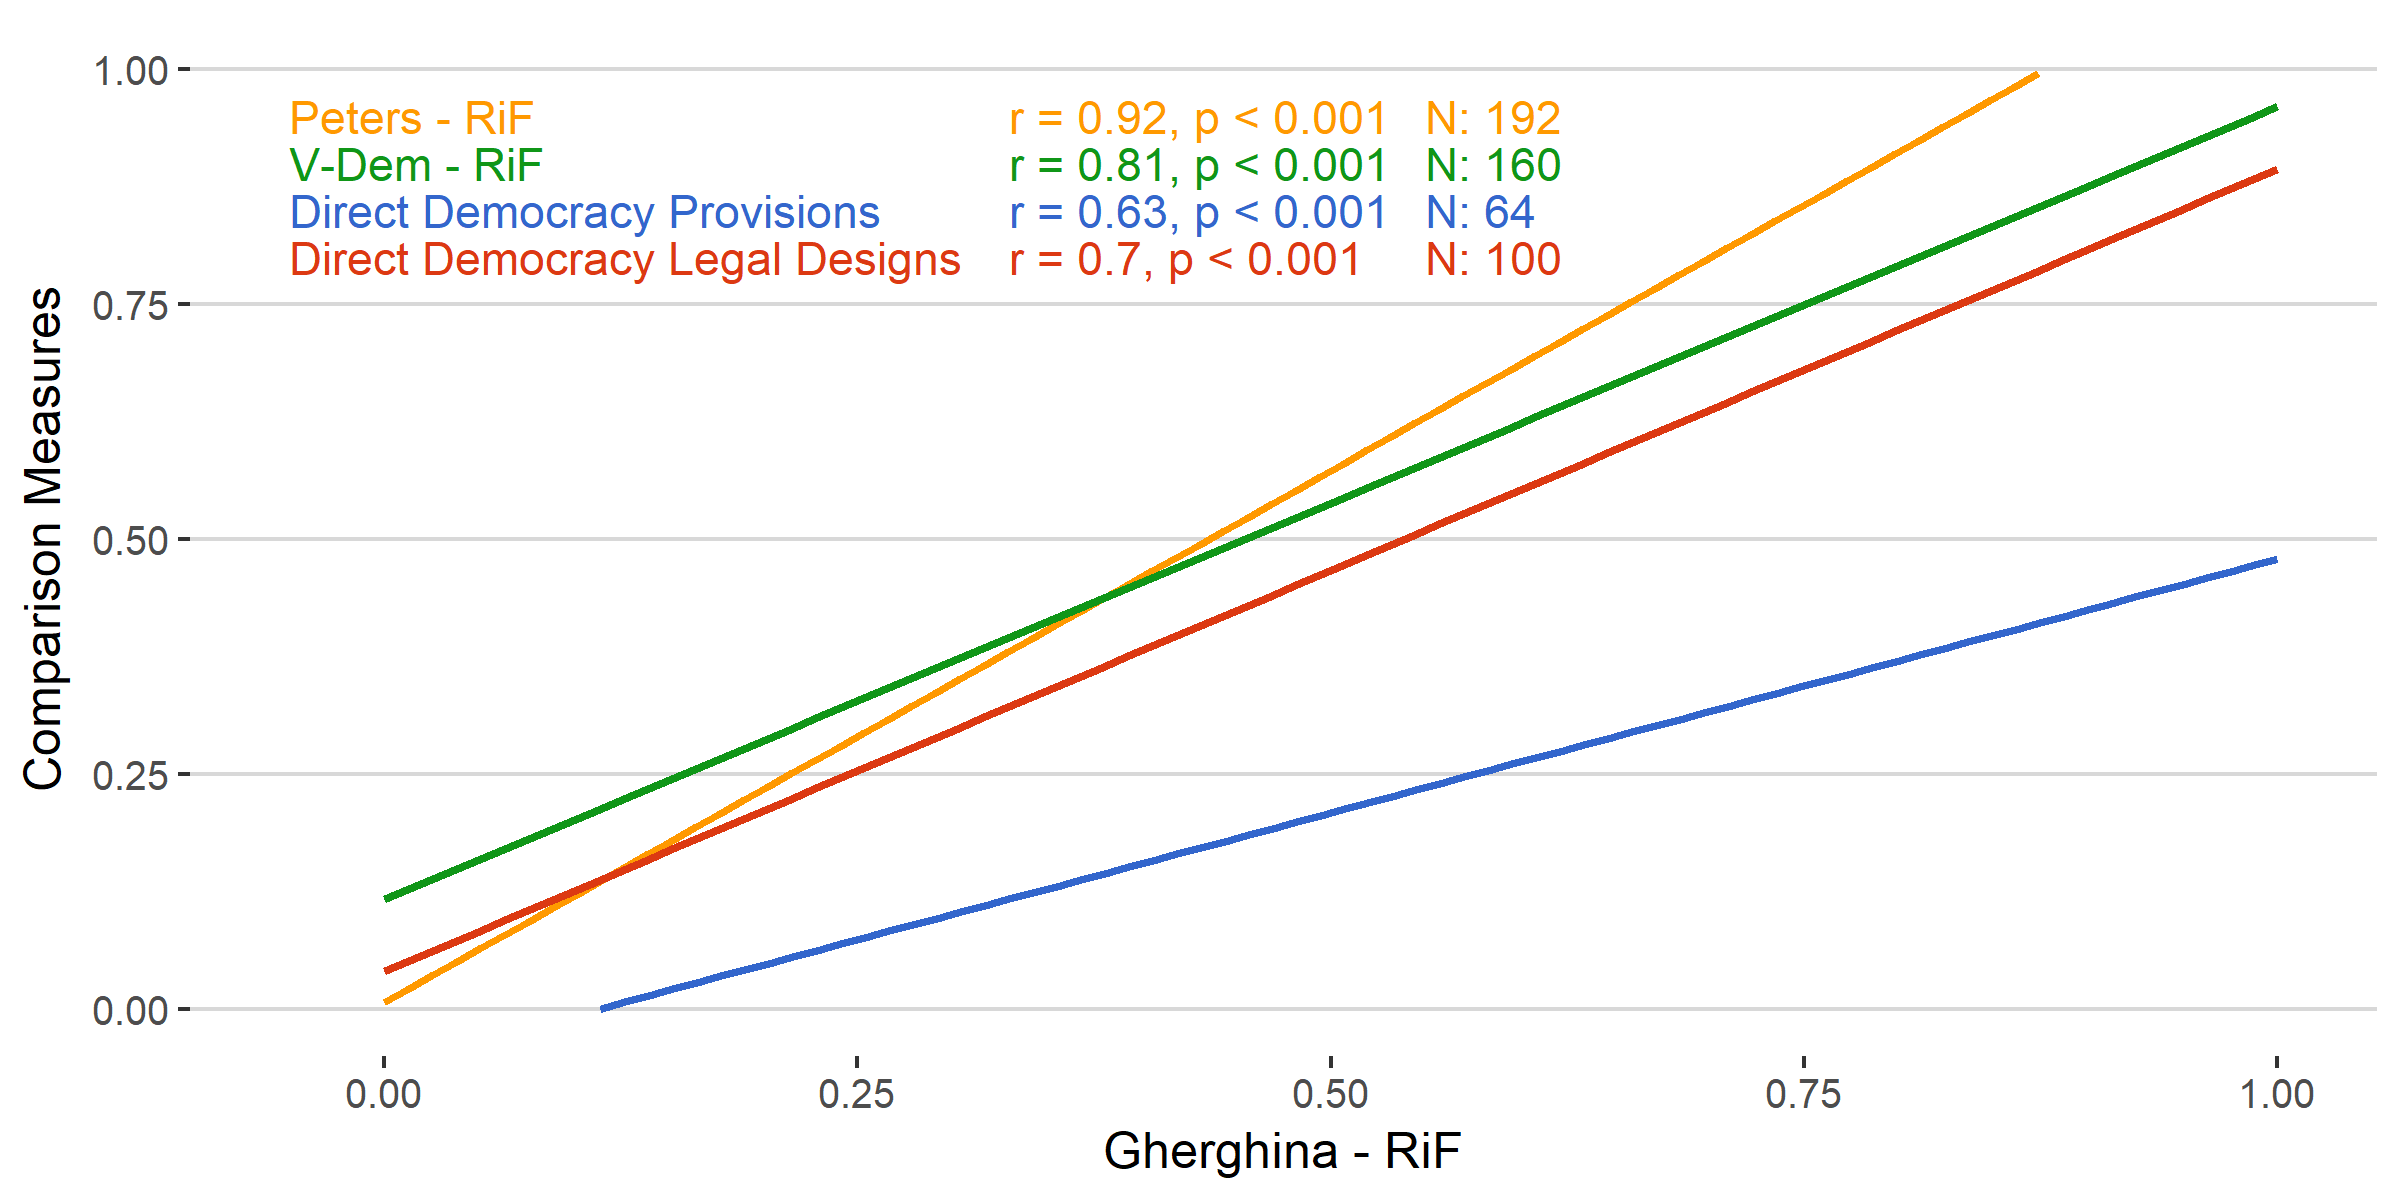
\includegraphics[width=\textwidth]{images/rif_ghergina.png}
	\flushright
	{\scriptsize $^{***}p<0.001$, $^{**}p<0.01$, $^*p<0.05$, $^{\dagger}p<0.1$. Standardized regression coefficients and 90\% confidence intervals are reported. For the full models see Appendix \ref{mod3}. Data weighted to same sample size (=1000). Data Source: see Table \ref{data} in the Appendix. Own calculations  \par}
\end{figure}

This is not very surprising, as they are both reconstructed using IDEA data, even though Gherghina also considers the recall institution, while the Peters measures gives different weights to each institution and accounts for bindingness. The count measure constructed on the basis of the V-Dem mechanisms (V-Dem RiF) is also closely associated with the Gherghina index (r = 0.81), as well as the Peters measure (r = 0.78). The Direct Democracy Provisions measure by the Democracy Barometer is also rather strongly related to both measures, although systematically smaller values can be observed (r > 0.6). This could be explained by the differing underlying typology, the different data collection, the fact that ease of approval is accounted for as well as the consideration of only binding mechanisms. Rather strong correlations can also be observed with the Direct Democracy Legal Designs variable, which is rather surprising given the fact that the data is partly incomplete and the completely different underlying definition of mechanisms (r > 0.5). 




\begin{figure}
	\caption{Peters RiF compared to other Rules in Form Measures}
	\label{reg2}
	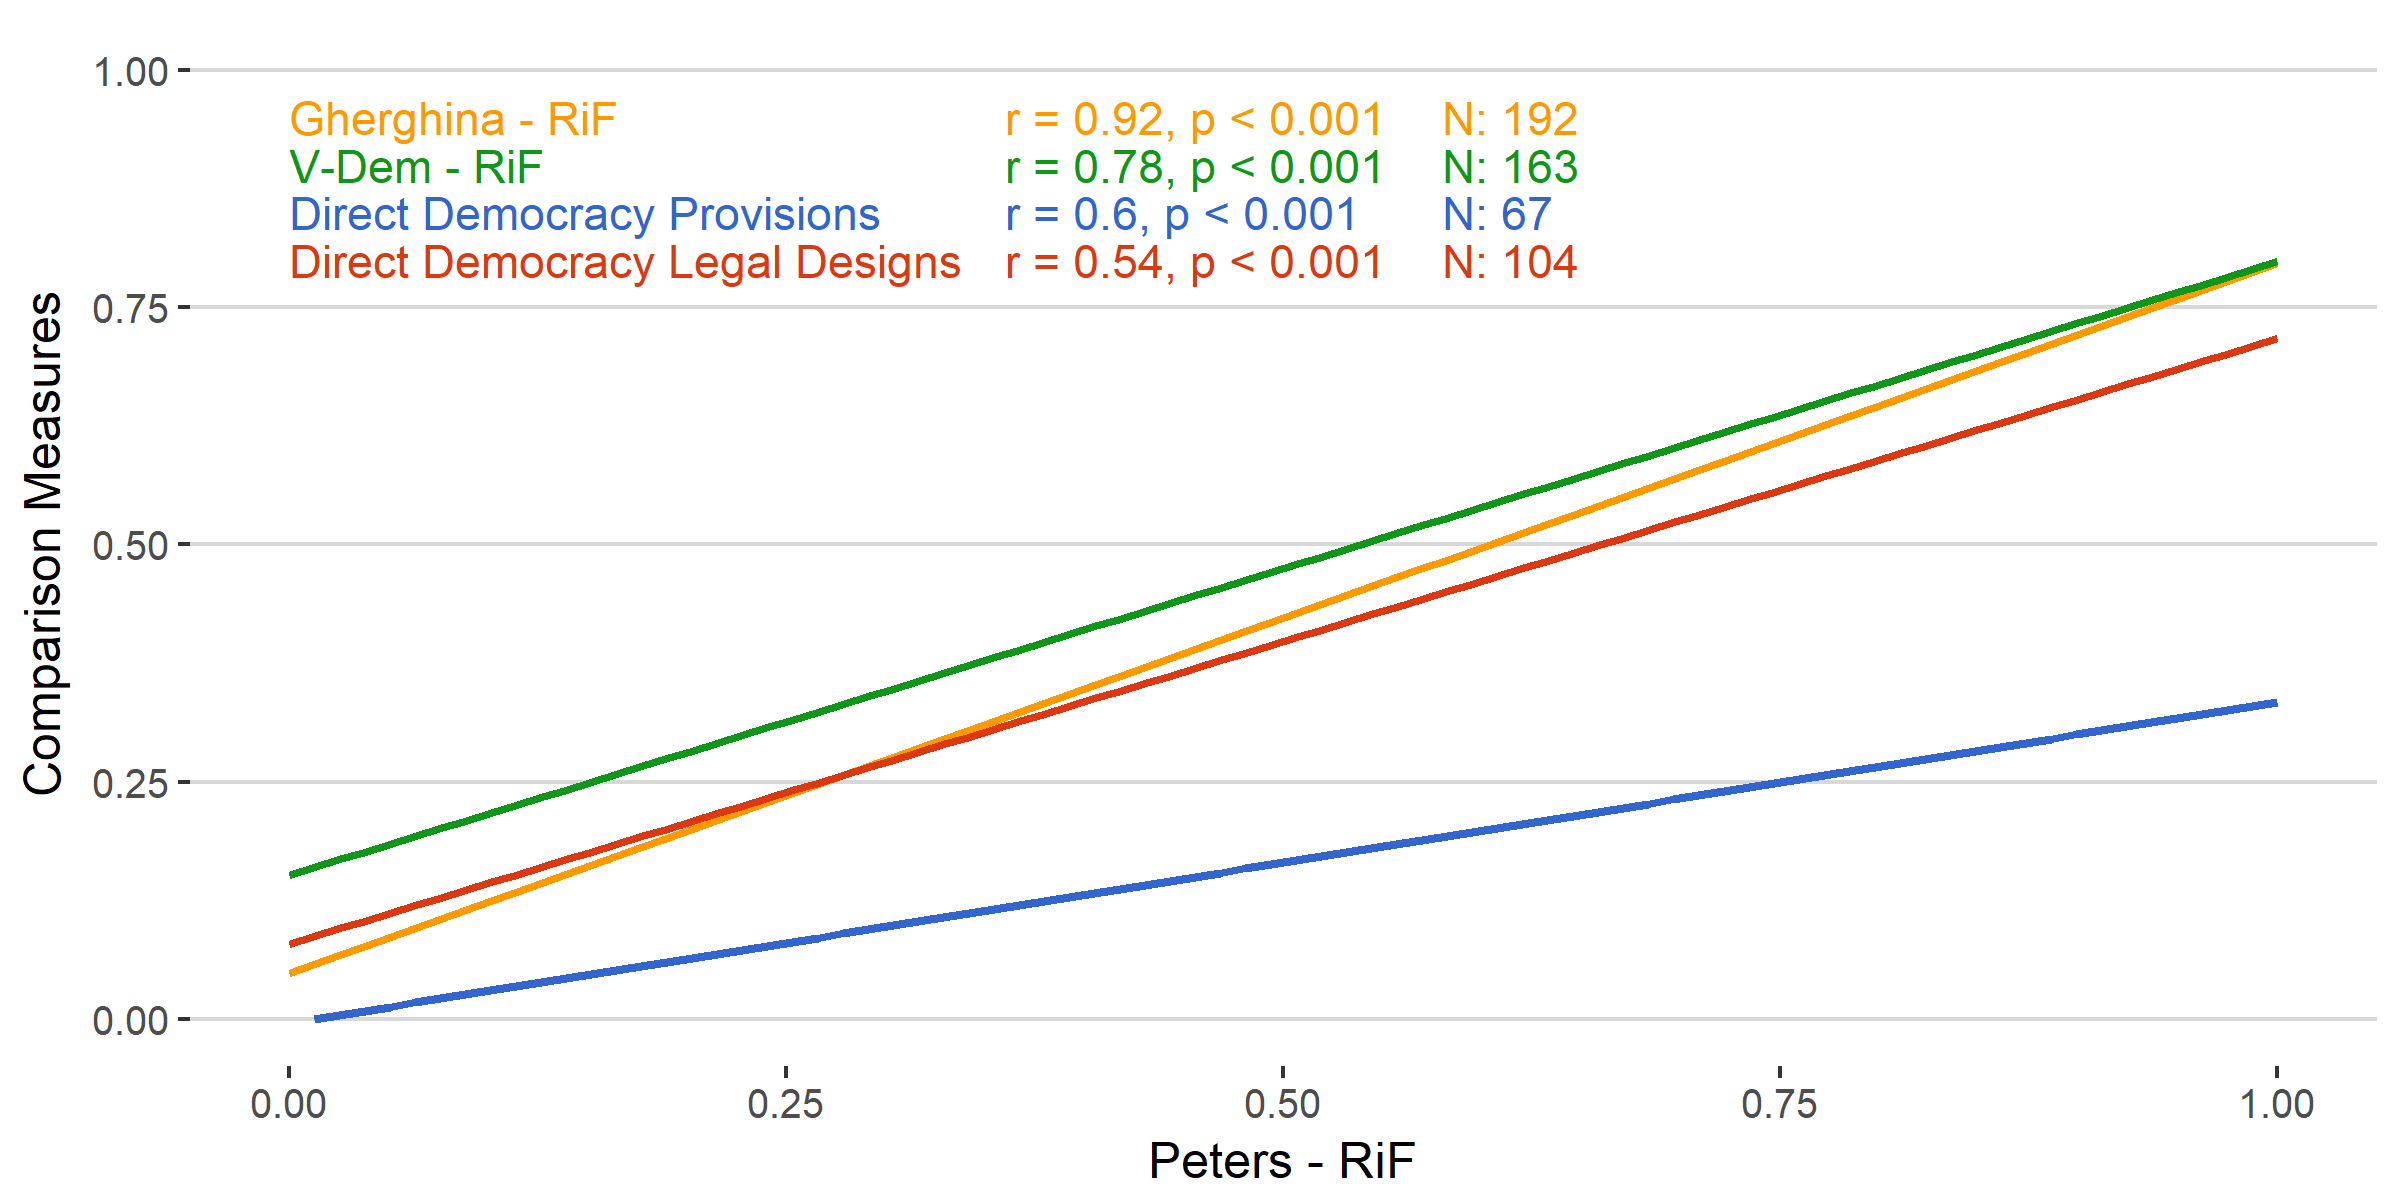
\includegraphics[width=\textwidth]{images/rif_peters.png}
	\flushright
	{\scriptsize $^{***}p<0.001$, $^{**}p<0.01$, $^*p<0.05$, $^{\dagger}p<0.1$. Standardized regression coefficients and 90\% confidence intervals are reported. For the full models see Appendix \ref{mod3}. Data weighted to same sample size (=1000). Data Source: see Table \ref{data} in the Appendix. Own calculations  \par}
\end{figure}



To get a better overview in regard to how the indices differ across regime types, we compare their distributions visualized with density plots (Figure XX), grouped according to the Freedom House classification into free, partly-free and not-free countries [for the construction of the Freedom House index and the classification see @fh2018freedom].  It has to be noted that the visualized distributions are rather smooth, though in case of discrete variables the original categories can be recognized at the peaks. Most of the rules in form measures are rather normally distributed, with many countries  reaching medium scores and few countries with high and low scores. Concerning not-free countries (if available), the distributions become more skewed, with less countries having higher values, a pattern which appears with all of the applicable measures.It becomes visible that the simple count variable of Legal Designs is not very accurate, as even less countries score on higher values. In general, partly free countries score as high or even higher as the ones categorized as free on all indicators. This implicates that the previously discussed importance of the level of democracy should not be neglected when comparing direct democracy across a wider range of countries. One might argue that, given equal direct popular vote mechanisms, a semi-democratic country is still less direct *democratic*, than a “full” democracy. Nevertheless, this pattern is a noteworthy discovery that should be investigated further by future research.

\begin{figure}
	\caption{Peters RiF compared to other Rules in Form Measures}
	\label{reg2}
	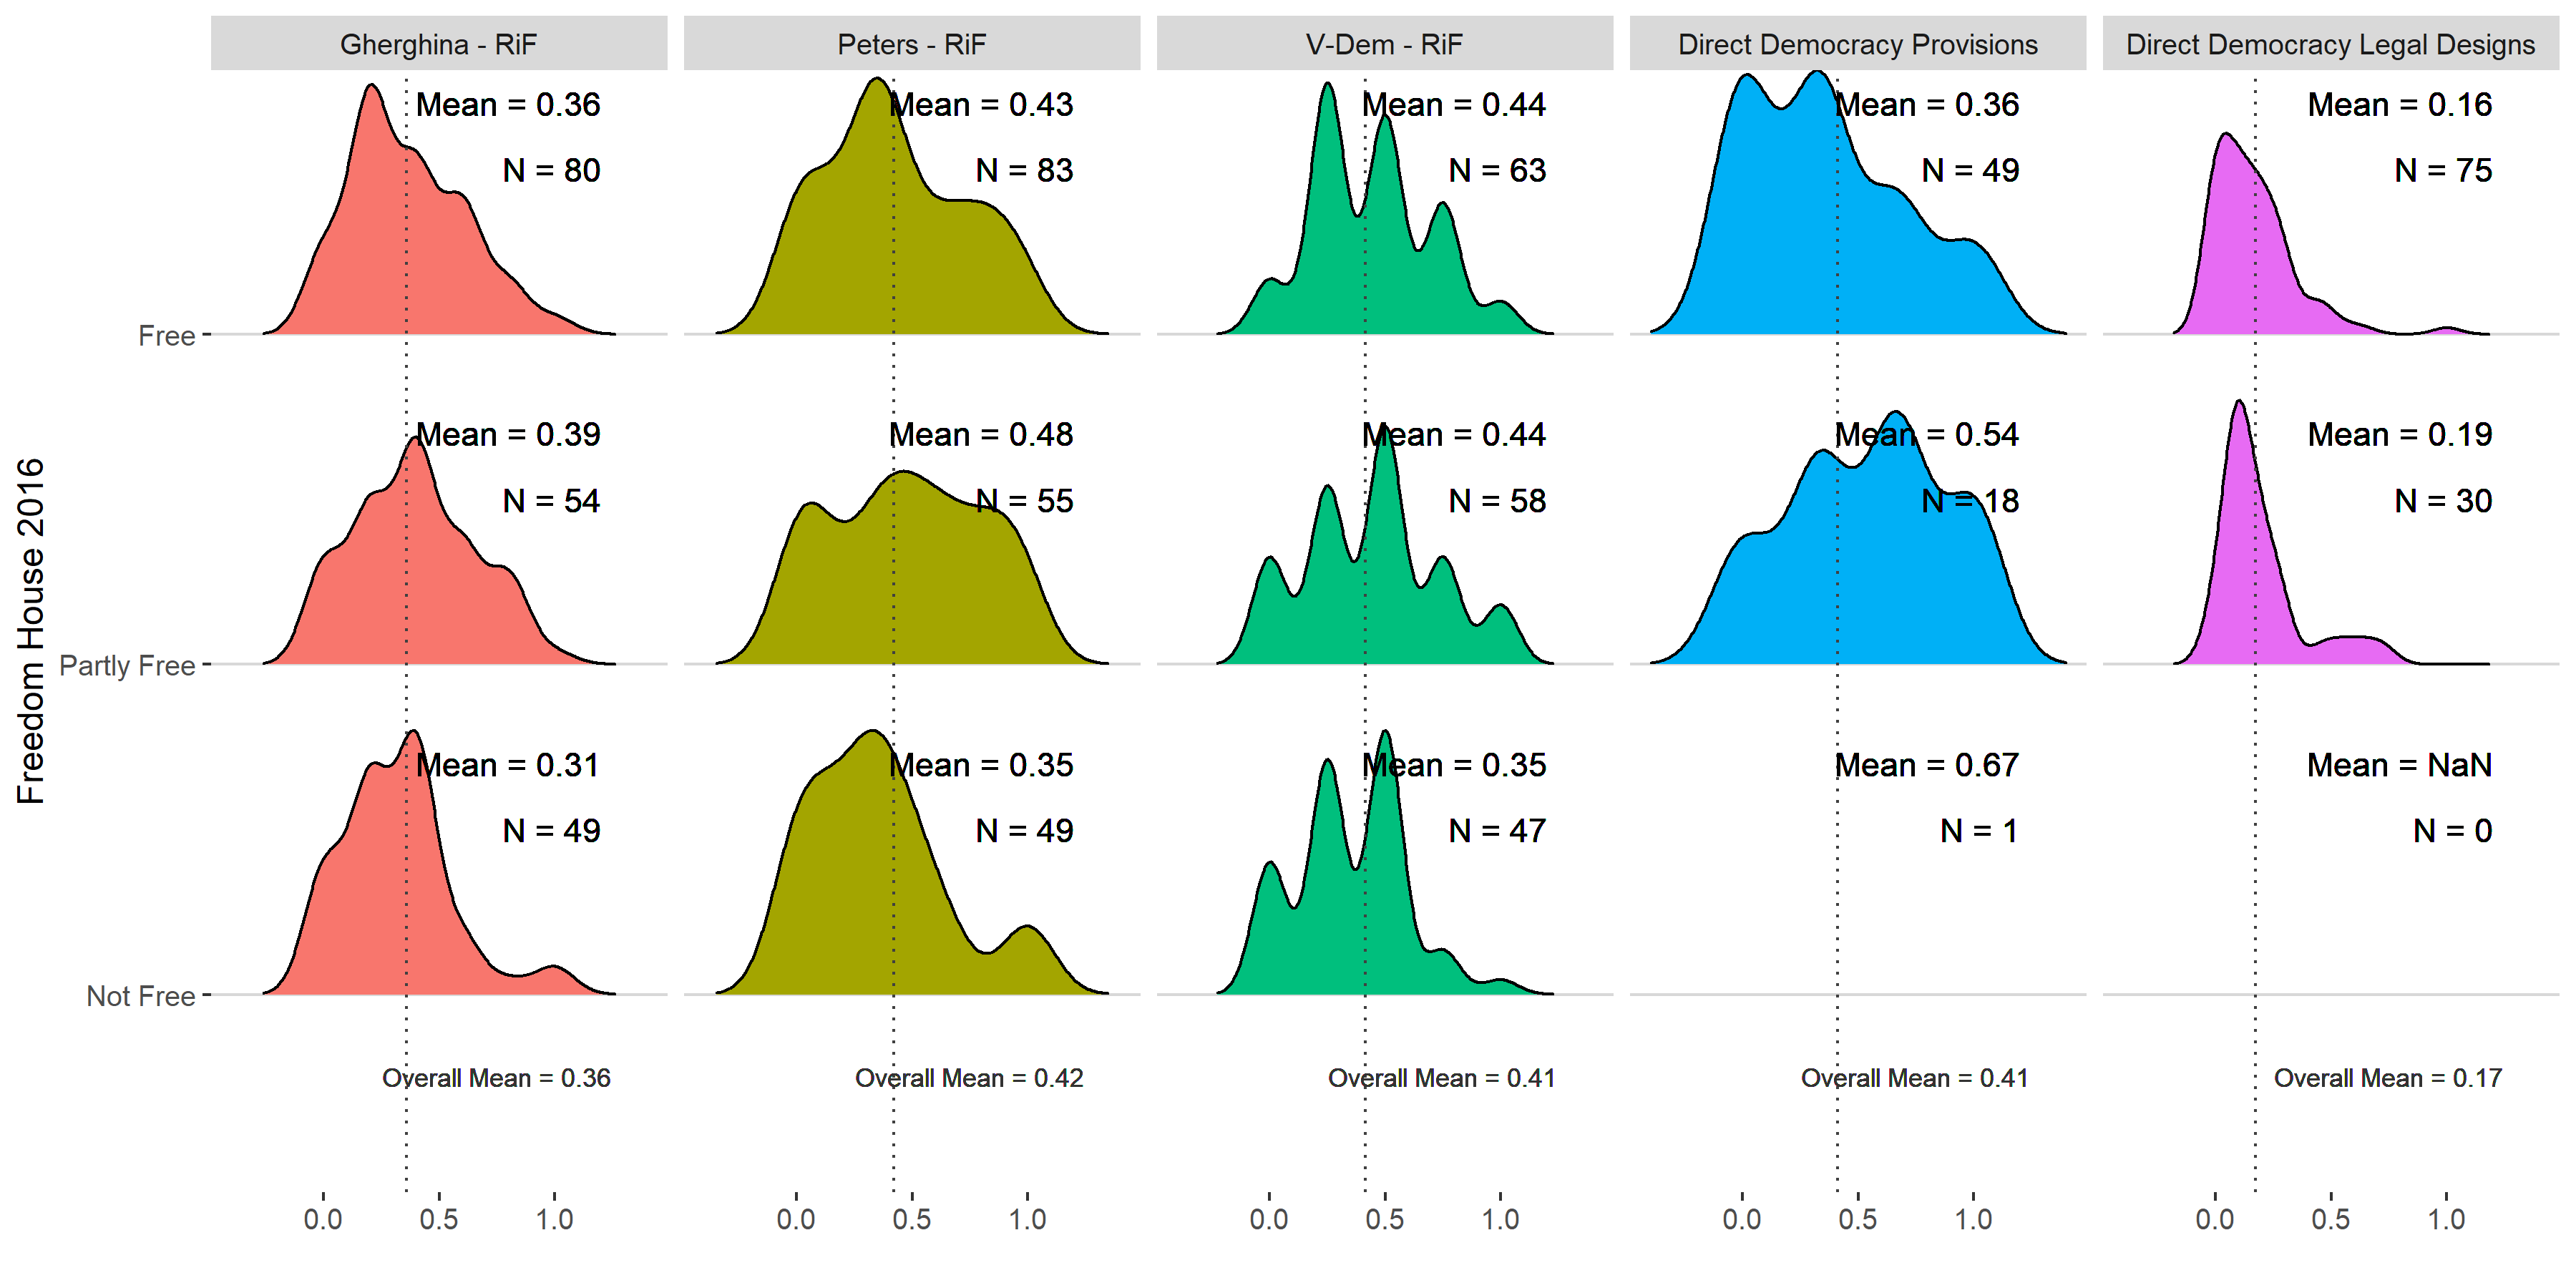
\includegraphics[width=\textwidth]{images/coef_rif2.png}
	\flushright
	{\scriptsize $^{***}p<0.001$, $^{**}p<0.01$, $^*p<0.05$, $^{\dagger}p<0.1$. Standardized regression coefficients and 90\% confidence intervals are reported. For the full models see Appendix \ref{mod3}. Data weighted to same sample size (=1000). Data Source: see Table \ref{data} in the Appendix. Own calculations  \par}
\end{figure}


Next, the distributions for the two bottom-up and top-down rules in form measures are depicted separately in Figure XX. Both indicators are rather similar, as they are both constructed using V-Dem data. It can be observed, that top-down provisions for direct democracy (Peters RiF Mean = 0.29; V-Dem RiF Mean = 0.53) are by far more common than citizen initiated institutions (Peters RiF Mean = 0.19; V-Dem RiF Mean = 0.63), which was already found by cf. @serdultwelp2012 pp. 77. Figure XX depicts a map, coloured according to a simple variable, indicating whether there are provisions only for bottom-up/ only for top down direct democratic mechanisms, for both or for none. Indication of such provisions is simply an index score above 0 on the respective measurement. 

\begin{figure}
	\caption{Peters RiF compared to other Rules in Form Measures}
	\label{reg2}
	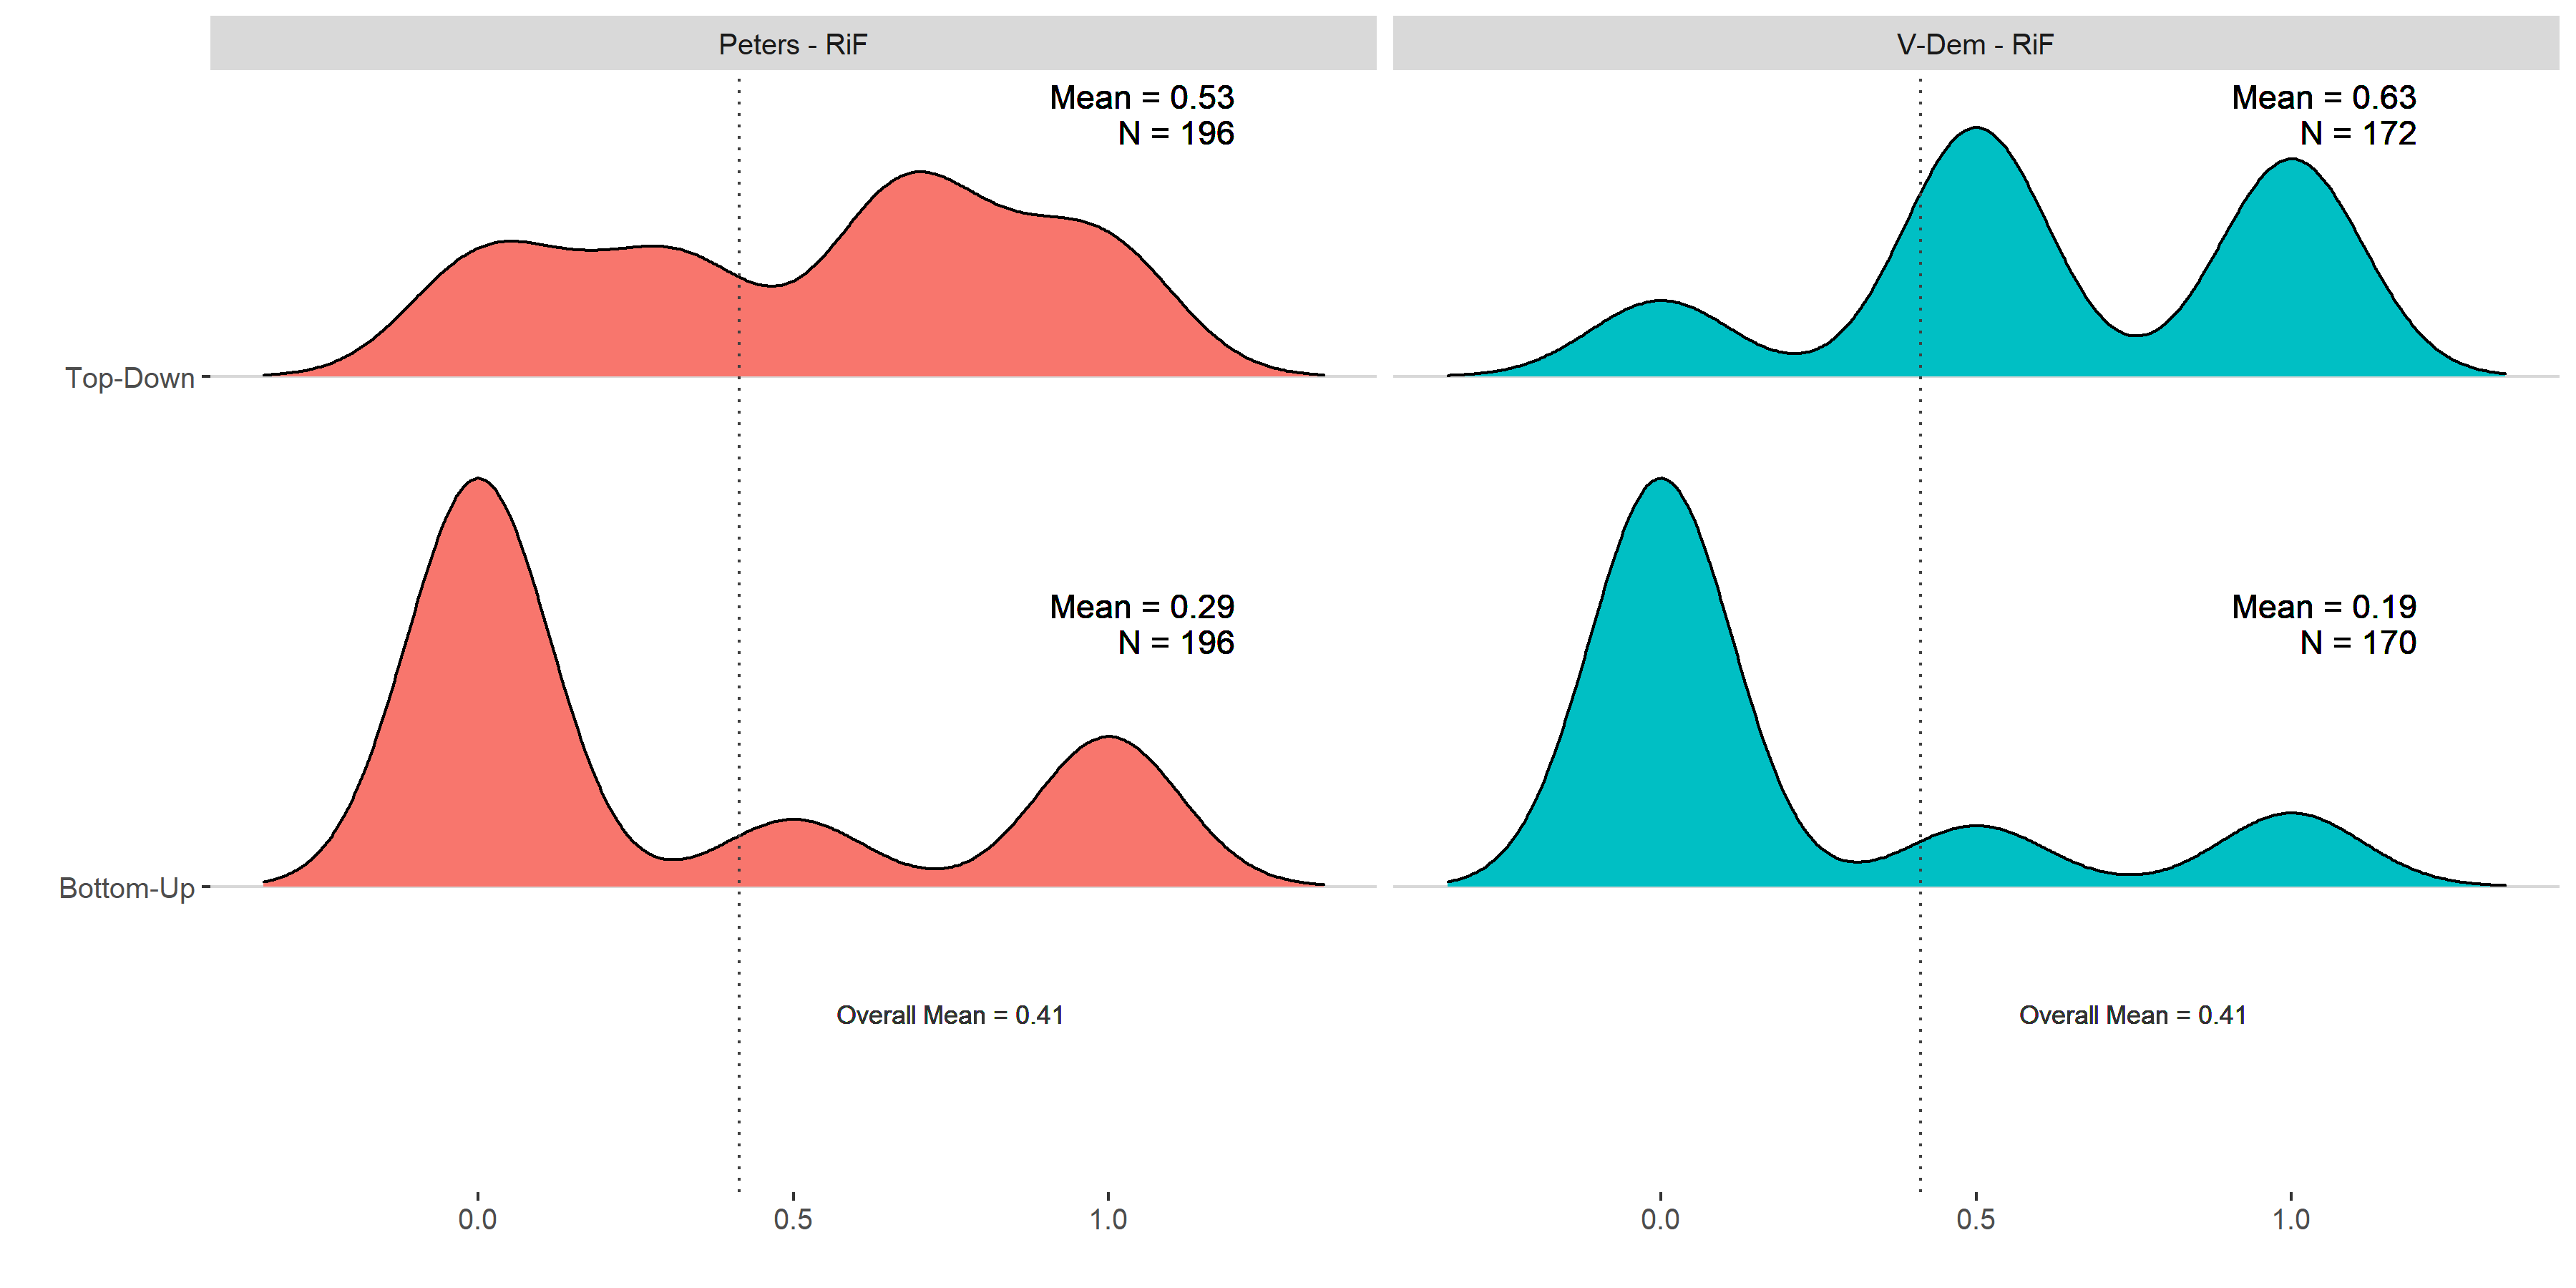
\includegraphics[width=\textwidth]{images/type_rif.png}
	\flushright
	{\scriptsize $^{***}p<0.001$, $^{**}p<0.01$, $^*p<0.05$, $^{\dagger}p<0.1$. Standardized regression coefficients and 90\% confidence intervals are reported. For the full models see Appendix \ref{mod3}. Data weighted to same sample size (=1000). Data Source: see Table \ref{data} in the Appendix. Own calculations  \par}
\end{figure}



Differences in classification are due to the consideration of different mechanisms, as well as different data sources for each measure. Here, the previous finding becomes apparent as well: a majority of countries only provide for top-down institutions (Peters - RiF N = 95; V-Dem RiF N = 106), while, depending on the coding scheme, a much smaller part has provisions for both (Peters - RiF N = 67; V-Dem RiF N = 42). Interestingly, but consistent with the literature, those countries can be found mostly in Eastern Europe and Latin America [cf. @ ]. There are 33 (Peters - RiF) or 24 (V-Dem - RiF) countries that provide neither top-down nor bottom-up mechanisms. Interestingly enough, there is a single case (the Netherlands) that has only bottom-up mechanisms in place, as indicated by the Peters - RiF measure.


\begin{figure}
\caption{Peters RiF compared to other Rules in Form Measures}
\label{reg2}
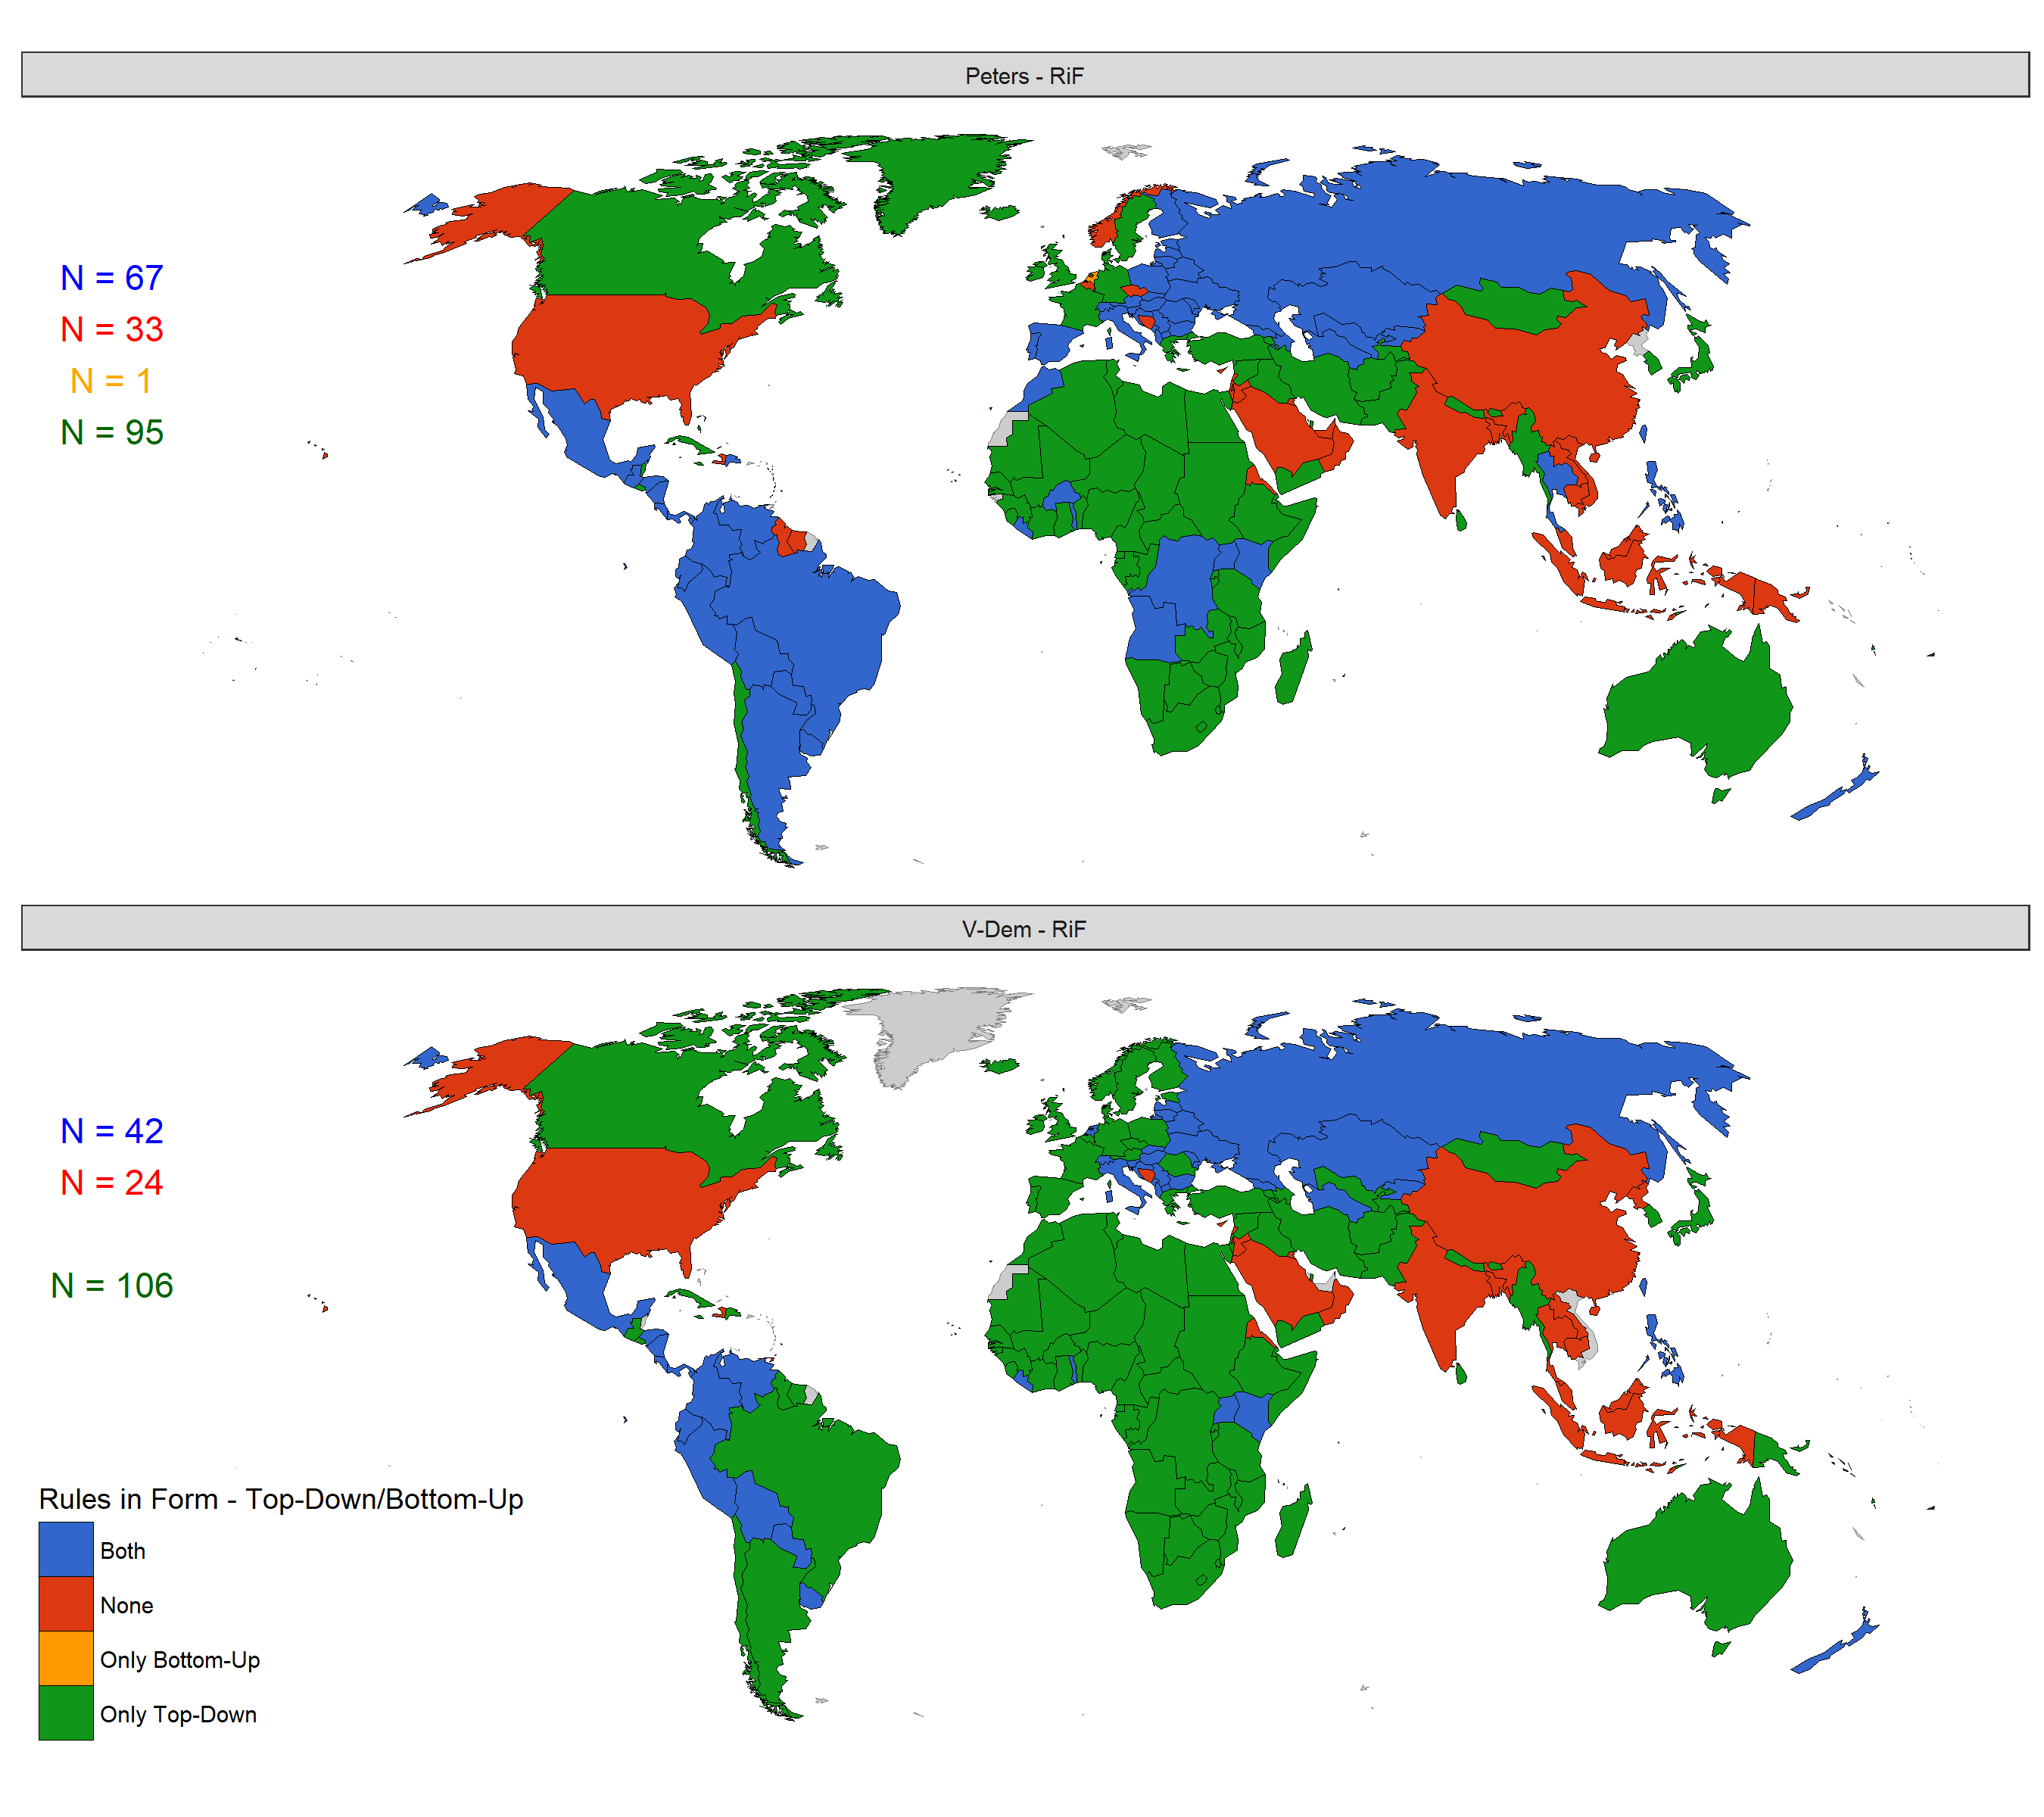
\includegraphics[width=\textwidth]{images/map_rif.png}
\flushright
{\scriptsize $^{***}p<0.001$, $^{**}p<0.01$, $^*p<0.05$, $^{\dagger}p<0.1$. Standardized regression coefficients and 90\% confidence intervals are reported. For the full models see Appendix \ref{mod3}. Data weighted to same sample size (=1000). Data Source: see Table \ref{data} in the Appendix. Own calculations  \par}
\end{figure}



\subsection{Comparing Rules in Use Measures}




As we examine even more rules in use indicators, only one approach is compared with the others, namely Gherghina - RiU, the measure constructed following @gherghina2016, as it differs the most in regard to construction (easiness of approval and decisiveness are accounted for). As most of the indices rely on some kind of count measure, and empirically there are many countries in which direct democracy is rarely used, but very few in which it is used extensively (the most prominent example being Switzerland, but also Uruguay and Azerbaijan stand out as outliers), we use the rank-based correlation coefficient Spearman’s Rho to account for the heavily skewed data. 

The summed up indicator based on V-Dem data shows the strongest relation to the Gherghina measure(Rho = 0.98), which was also constructed using V-Dem data (Figure XX). All the other indicators have strong correlations as well, the least being the Effective Use count measure (Rho = 0.65). In average, the indices seem to be in line with the Gherghina - RiU, although the  Sudd - RiU Sum as well as the Credible Use indicators are systematically observed at higher values.



\begin{figure}
	\caption{Peters RiF compared to other Rules in Form Measures}
	\label{reg2}
	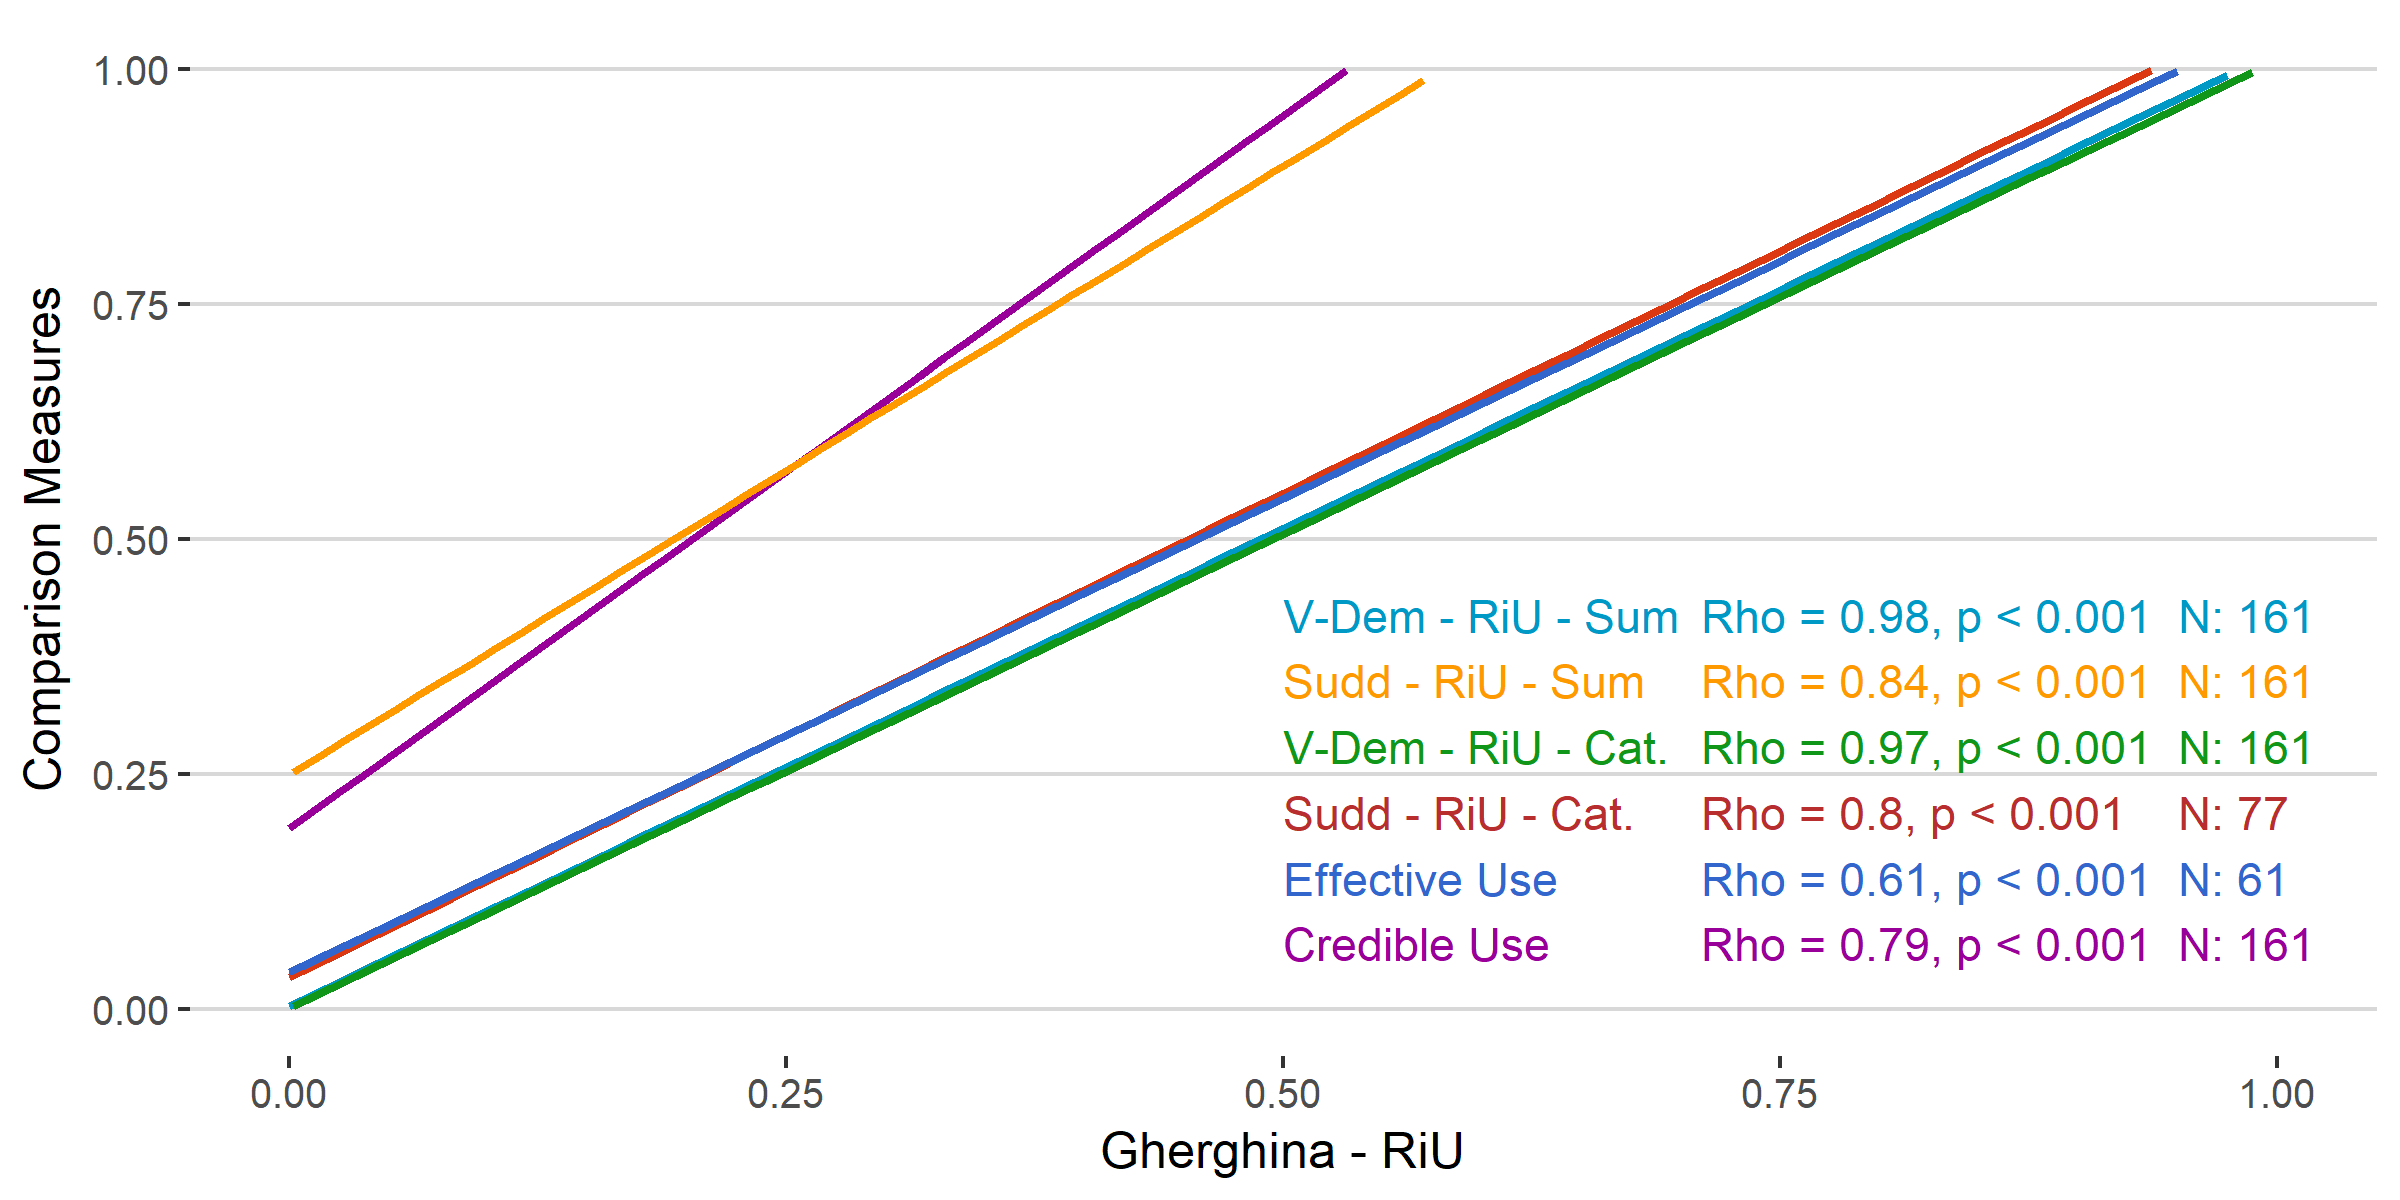
\includegraphics[width=\textwidth]{images/riu_ghergina.png}
	\flushright
	{\scriptsize $^{***}p<0.001$, $^{**}p<0.01$, $^*p<0.05$, $^{\dagger}p<0.1$. Standardized regression coefficients and 90\% confidence intervals are reported. For the full models see Appendix \ref{mod3}. Data weighted to same sample size (=1000). Data Source: see Table \ref{data} in the Appendix. Own calculations  \par}
\end{figure}

Figure XX depicts the distributions for the rules in use indicators, for which it can be observed that the summed up indicators, and also the Gherghina - RiU measure are heavily skewed, with very few countries ranging very high, while most are located at the lowest scores. Due to  construction, this does not apply as much to the Credible Use indicator, and even less to the categorical classifications, illustrating an important advantage of such measurement approaches, even if it implies a loss of empirical information. 

\begin{figure}
	\caption{Peters RiF compared to other Rules in Form Measures}
	\label{reg2}
	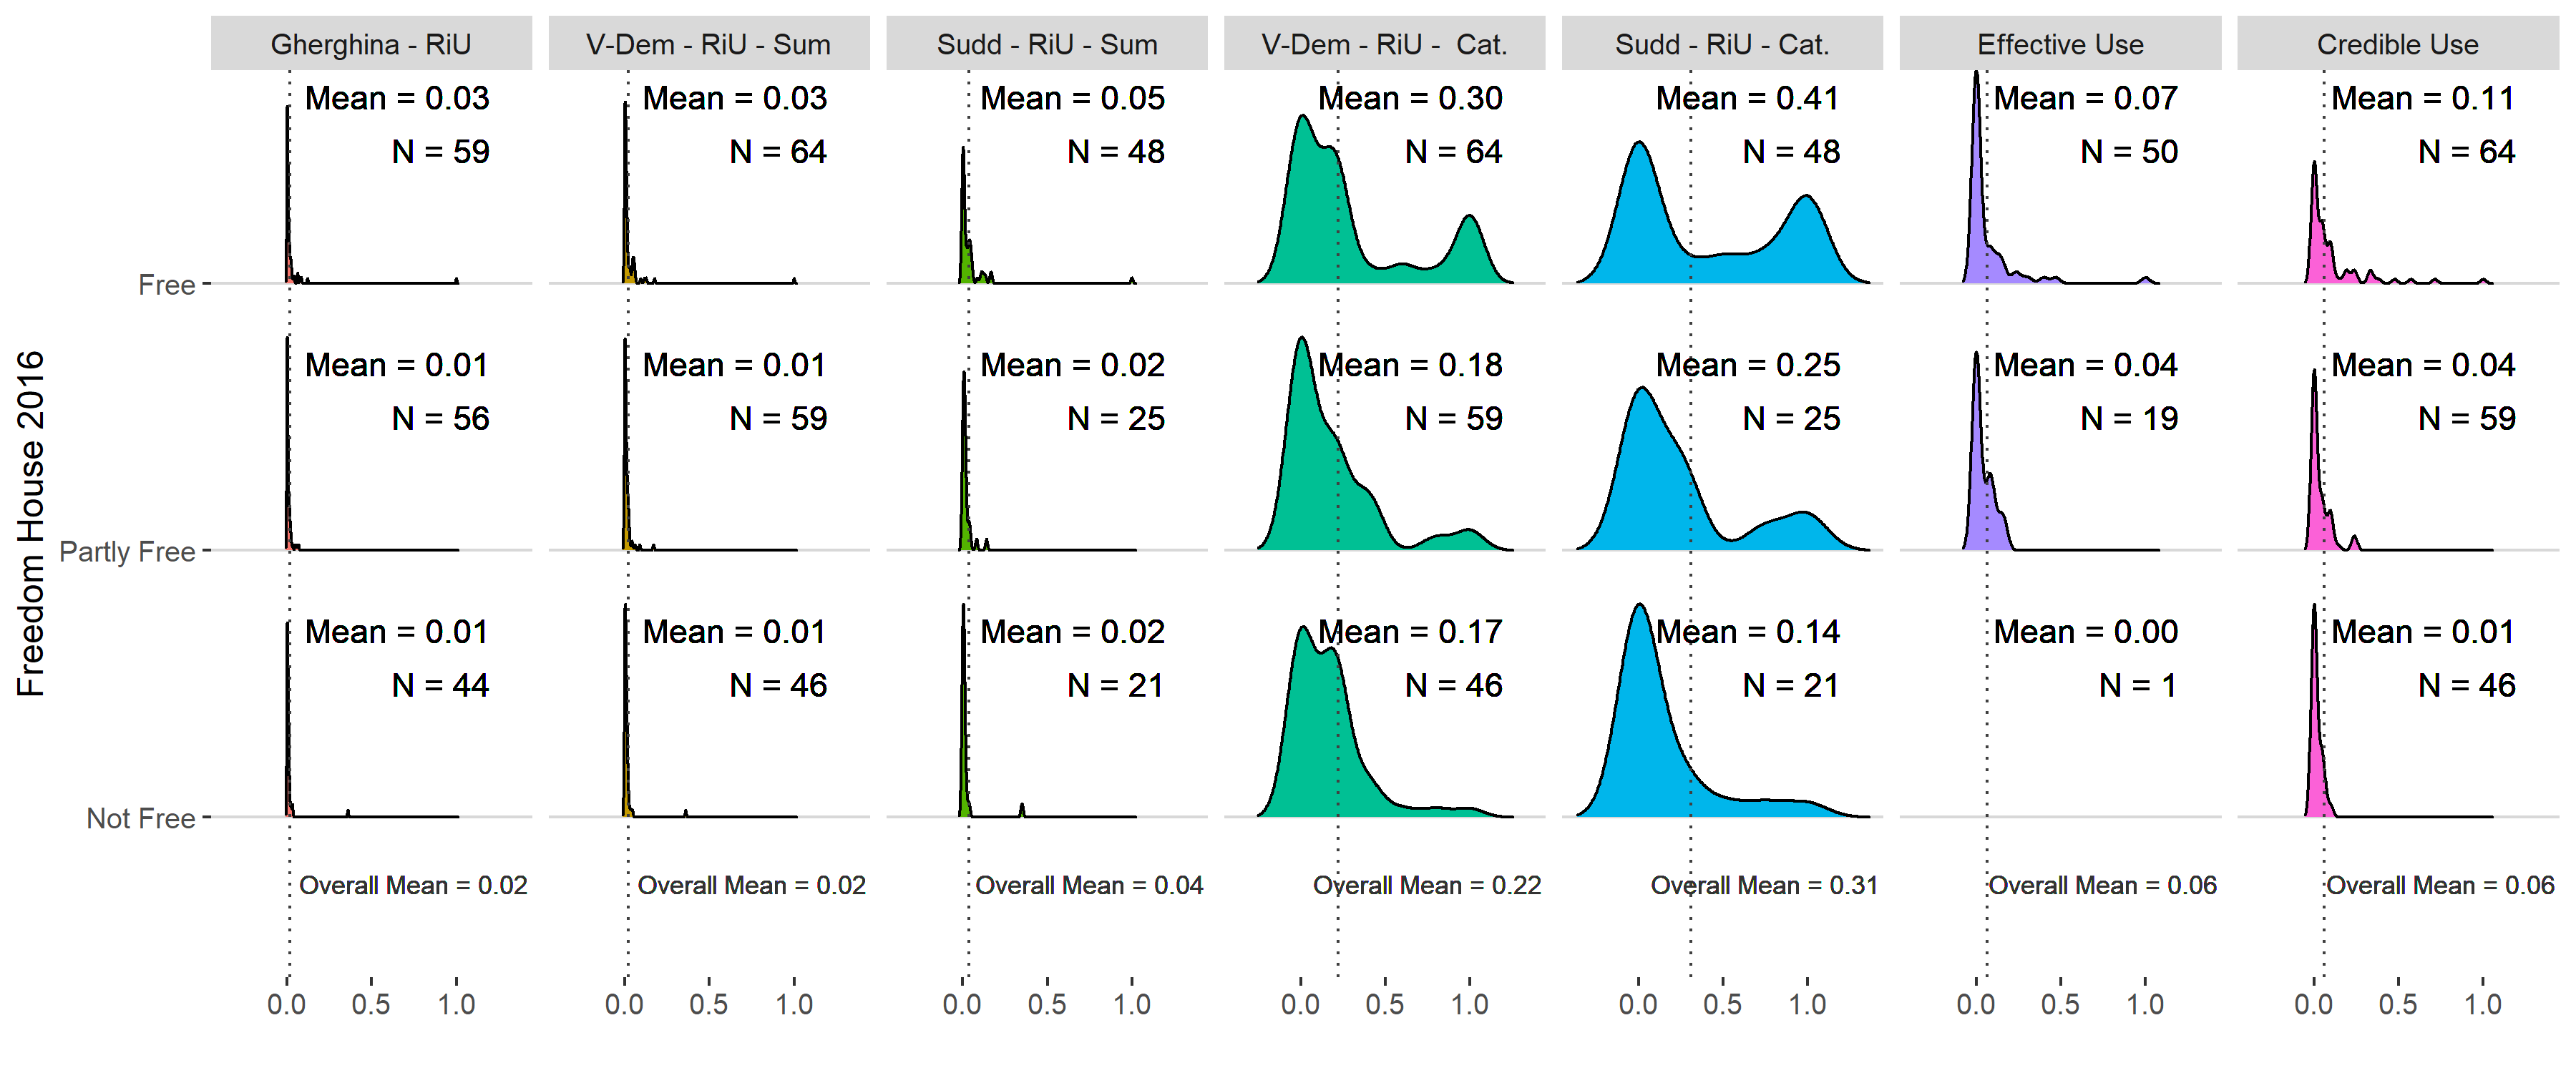
\includegraphics[width=\textwidth]{images/coef_riu2.png}
	\flushright
	{\scriptsize $^{***}p<0.001$, $^{**}p<0.01$, $^*p<0.05$, $^{\dagger}p<0.1$. Standardized regression coefficients and 90\% confidence intervals are reported. For the full models see Appendix \ref{mod3}. Data weighted to same sample size (=1000). Data Source: see Table \ref{data} in the Appendix. Own calculations  \par}
\end{figure}

In Figure XX, the categorial variables for top-down and bottom-up rules in use are depicted. For the V-Dem - RiU Categorized measure, it is evident that mostly top-down mechanisms are used in practice (Mean = 0.19) , while bottom-up mechanisms remain mainly unused (Mean = 0.05), wich was also observed by @serdultwelp2012 pp. 78. Of course, this is partially due to the fact that top-down mechanisms are much less common as rules in form, and citizens can’t use bottom-up mechanisms if they are not provided.  On the contrary, the Sudd - RiU Categorized measure implies an opposite trend: bottom-up usage has a mean of 0.40, while top-down usage has a mean of 0.24. However, this discrepancy arises from the structure of the sudd data, that only records direct democracy mechanisms that actually occurred. Correctly interpreted it can be said fewer bottom-up measures have taken place (N = 23) compared to top-down measures (N = 92), however in the countries where they did occur, they often occur quite frequently.

\begin{figure}
	\caption{Peters RiF compared to other Rules in Form Measures}
	\label{reg2}
	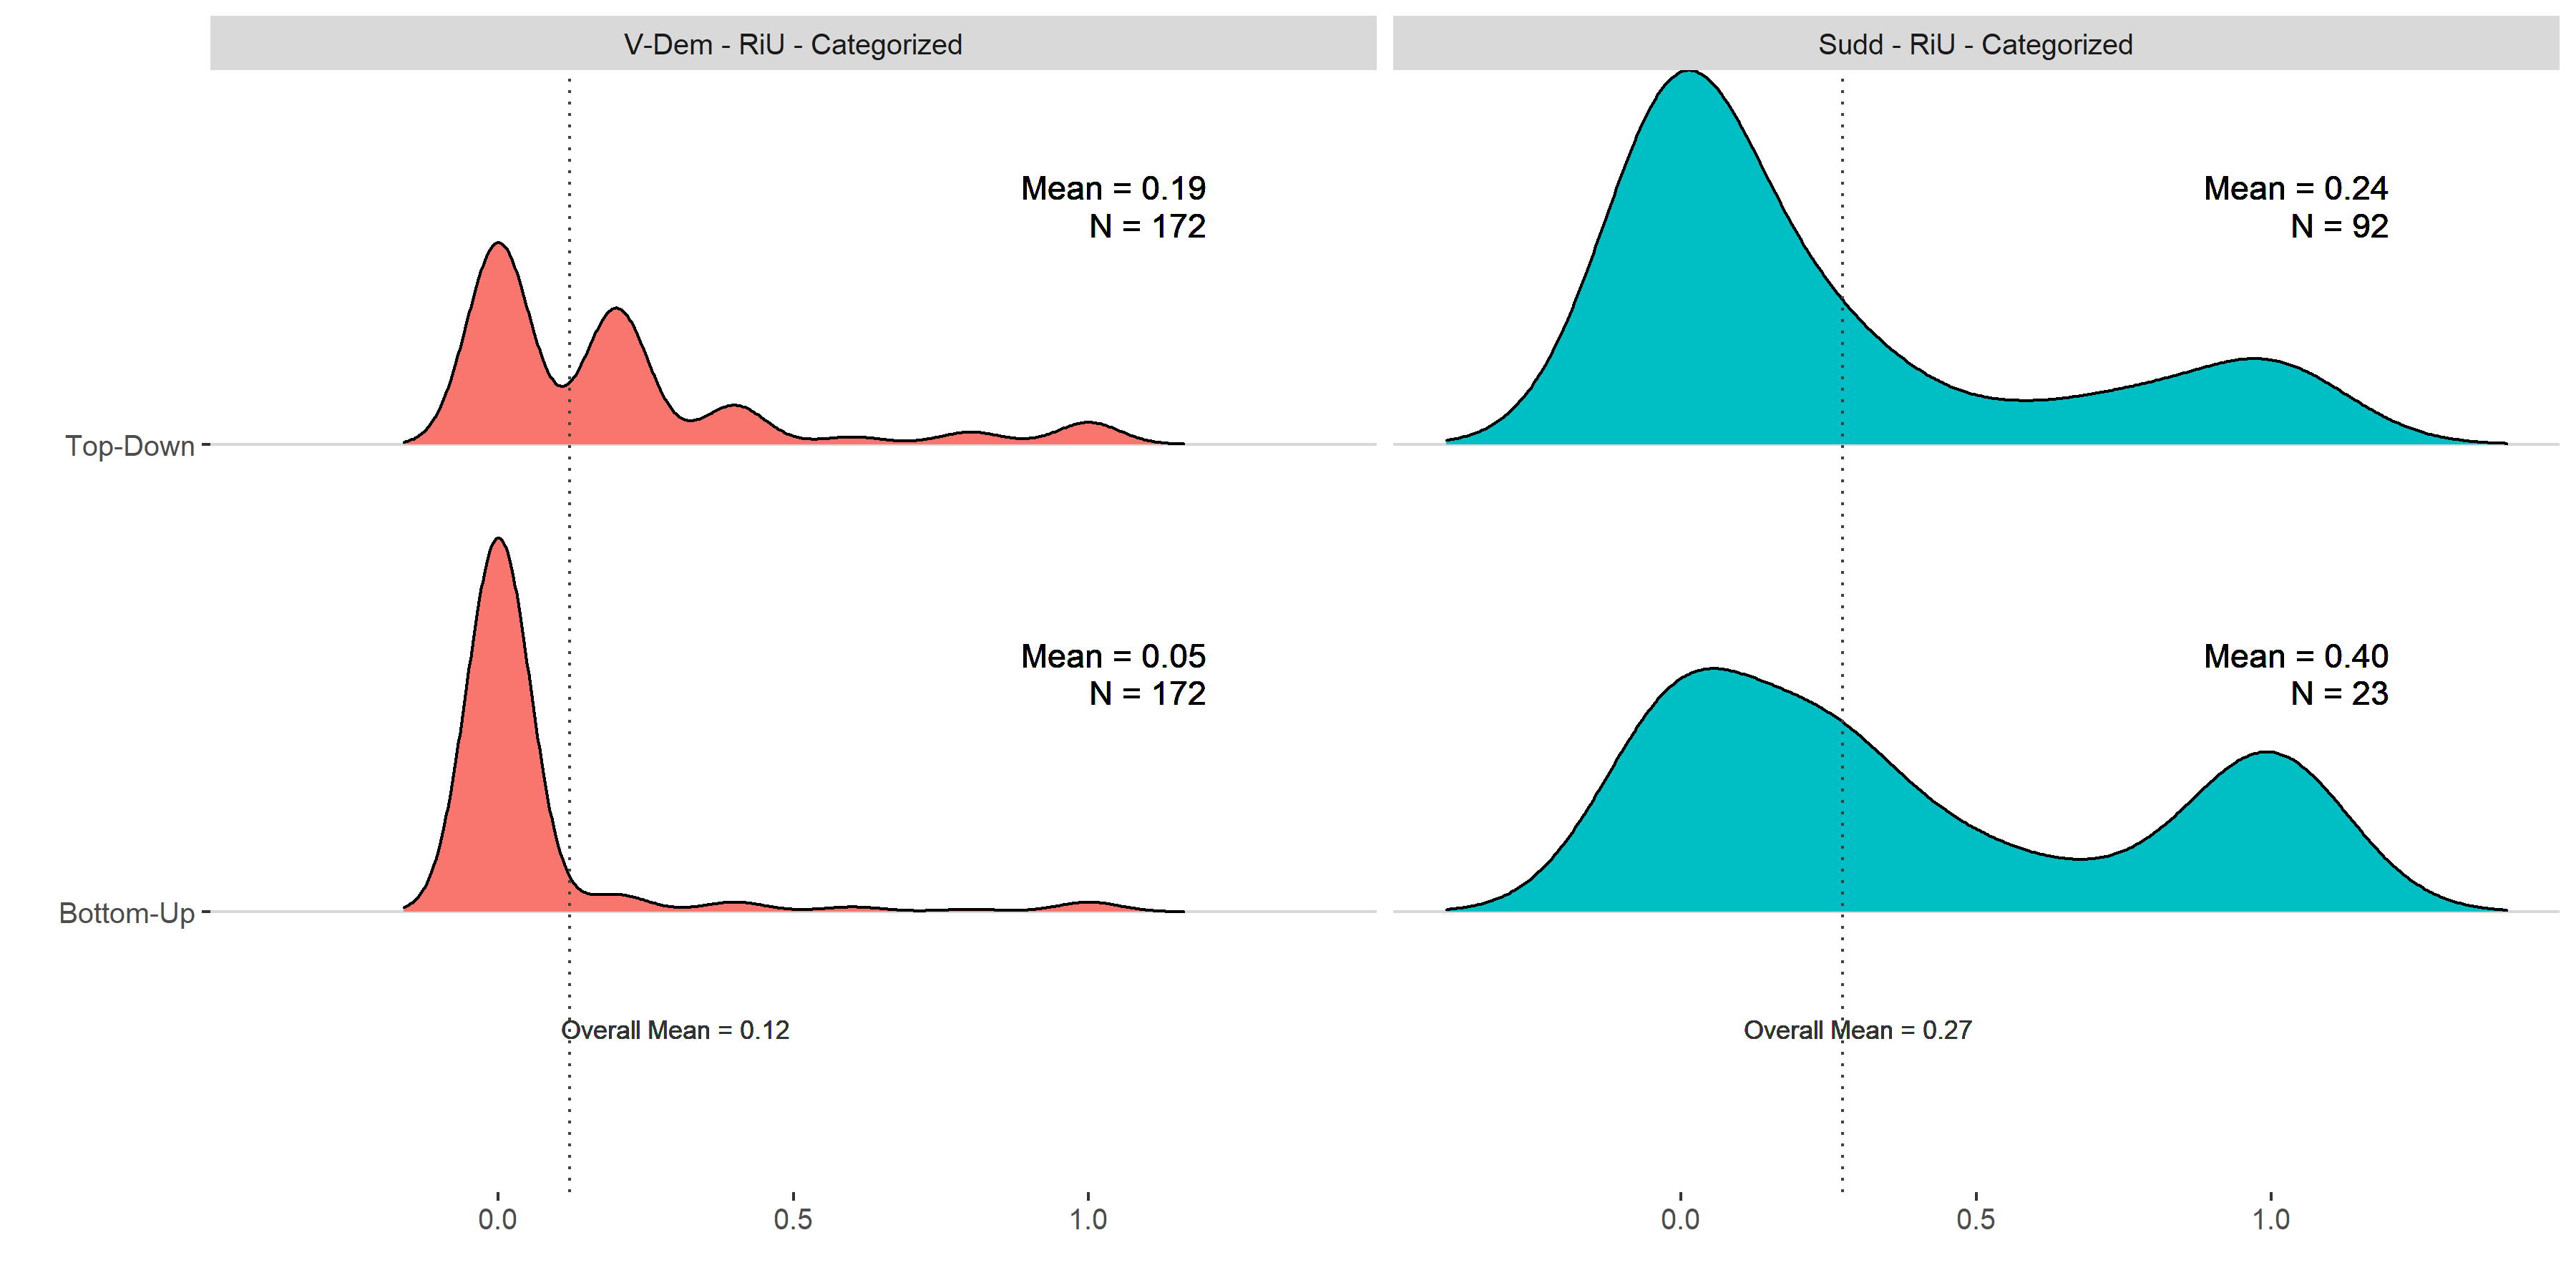
\includegraphics[width=\textwidth]{images/type_riu.png}
	\flushright
	{\scriptsize $^{***}p<0.001$, $^{**}p<0.01$, $^*p<0.05$, $^{\dagger}p<0.1$. Standardized regression coefficients and 90\% confidence intervals are reported. For the full models see Appendix \ref{mod3}. Data weighted to same sample size (=1000). Data Source: see Table \ref{data} in the Appendix. Own calculations  \par}
\end{figure}


Similar to the map depicting rules in form, Figure XX depicts a world map indicating whether, a country had at least one occurrence of only top-down or bottom up direct popular votes in between 1996 and 2016, or whether both occured at least once. As discussed before, the sudd dataset only embodies countries with at least one occurrence, which becomes obvious in comparison with the V-Dem measure. Most countries are assigned to the same category, for example both measures show that Ukraine, Macedonia and Peru are the three countries where only bottom-up measures occured. A  few exceptions can also be noted, for example Bolivia, which had only a top-down occurrence according to sudd, while V-Dem counts both top-down and bottom-up rules in use. In line with the previously described results, the biggest group consists of countries that used neither bottom-up nor top-down direct democracy (V-Dem - RiU N = 80), following such countries in which only top-down mechanisms are used (Sudd - RiU N = 72; V-Dem - RiU N = 74). Countries in which both mechanisms were used (Sudd - RiU N = 20; V-Dem - RiU N = 15) are mostly centered in Europe, while in Africa and Latin America mostly top-down mechanisms are practiced exclusively (which is not very surprising, as many countries in this regions only provide for such mechanisms).

\begin{figure}
	\caption{Peters RiF compared to other Rules in Form Measures}
	\label{reg2}
	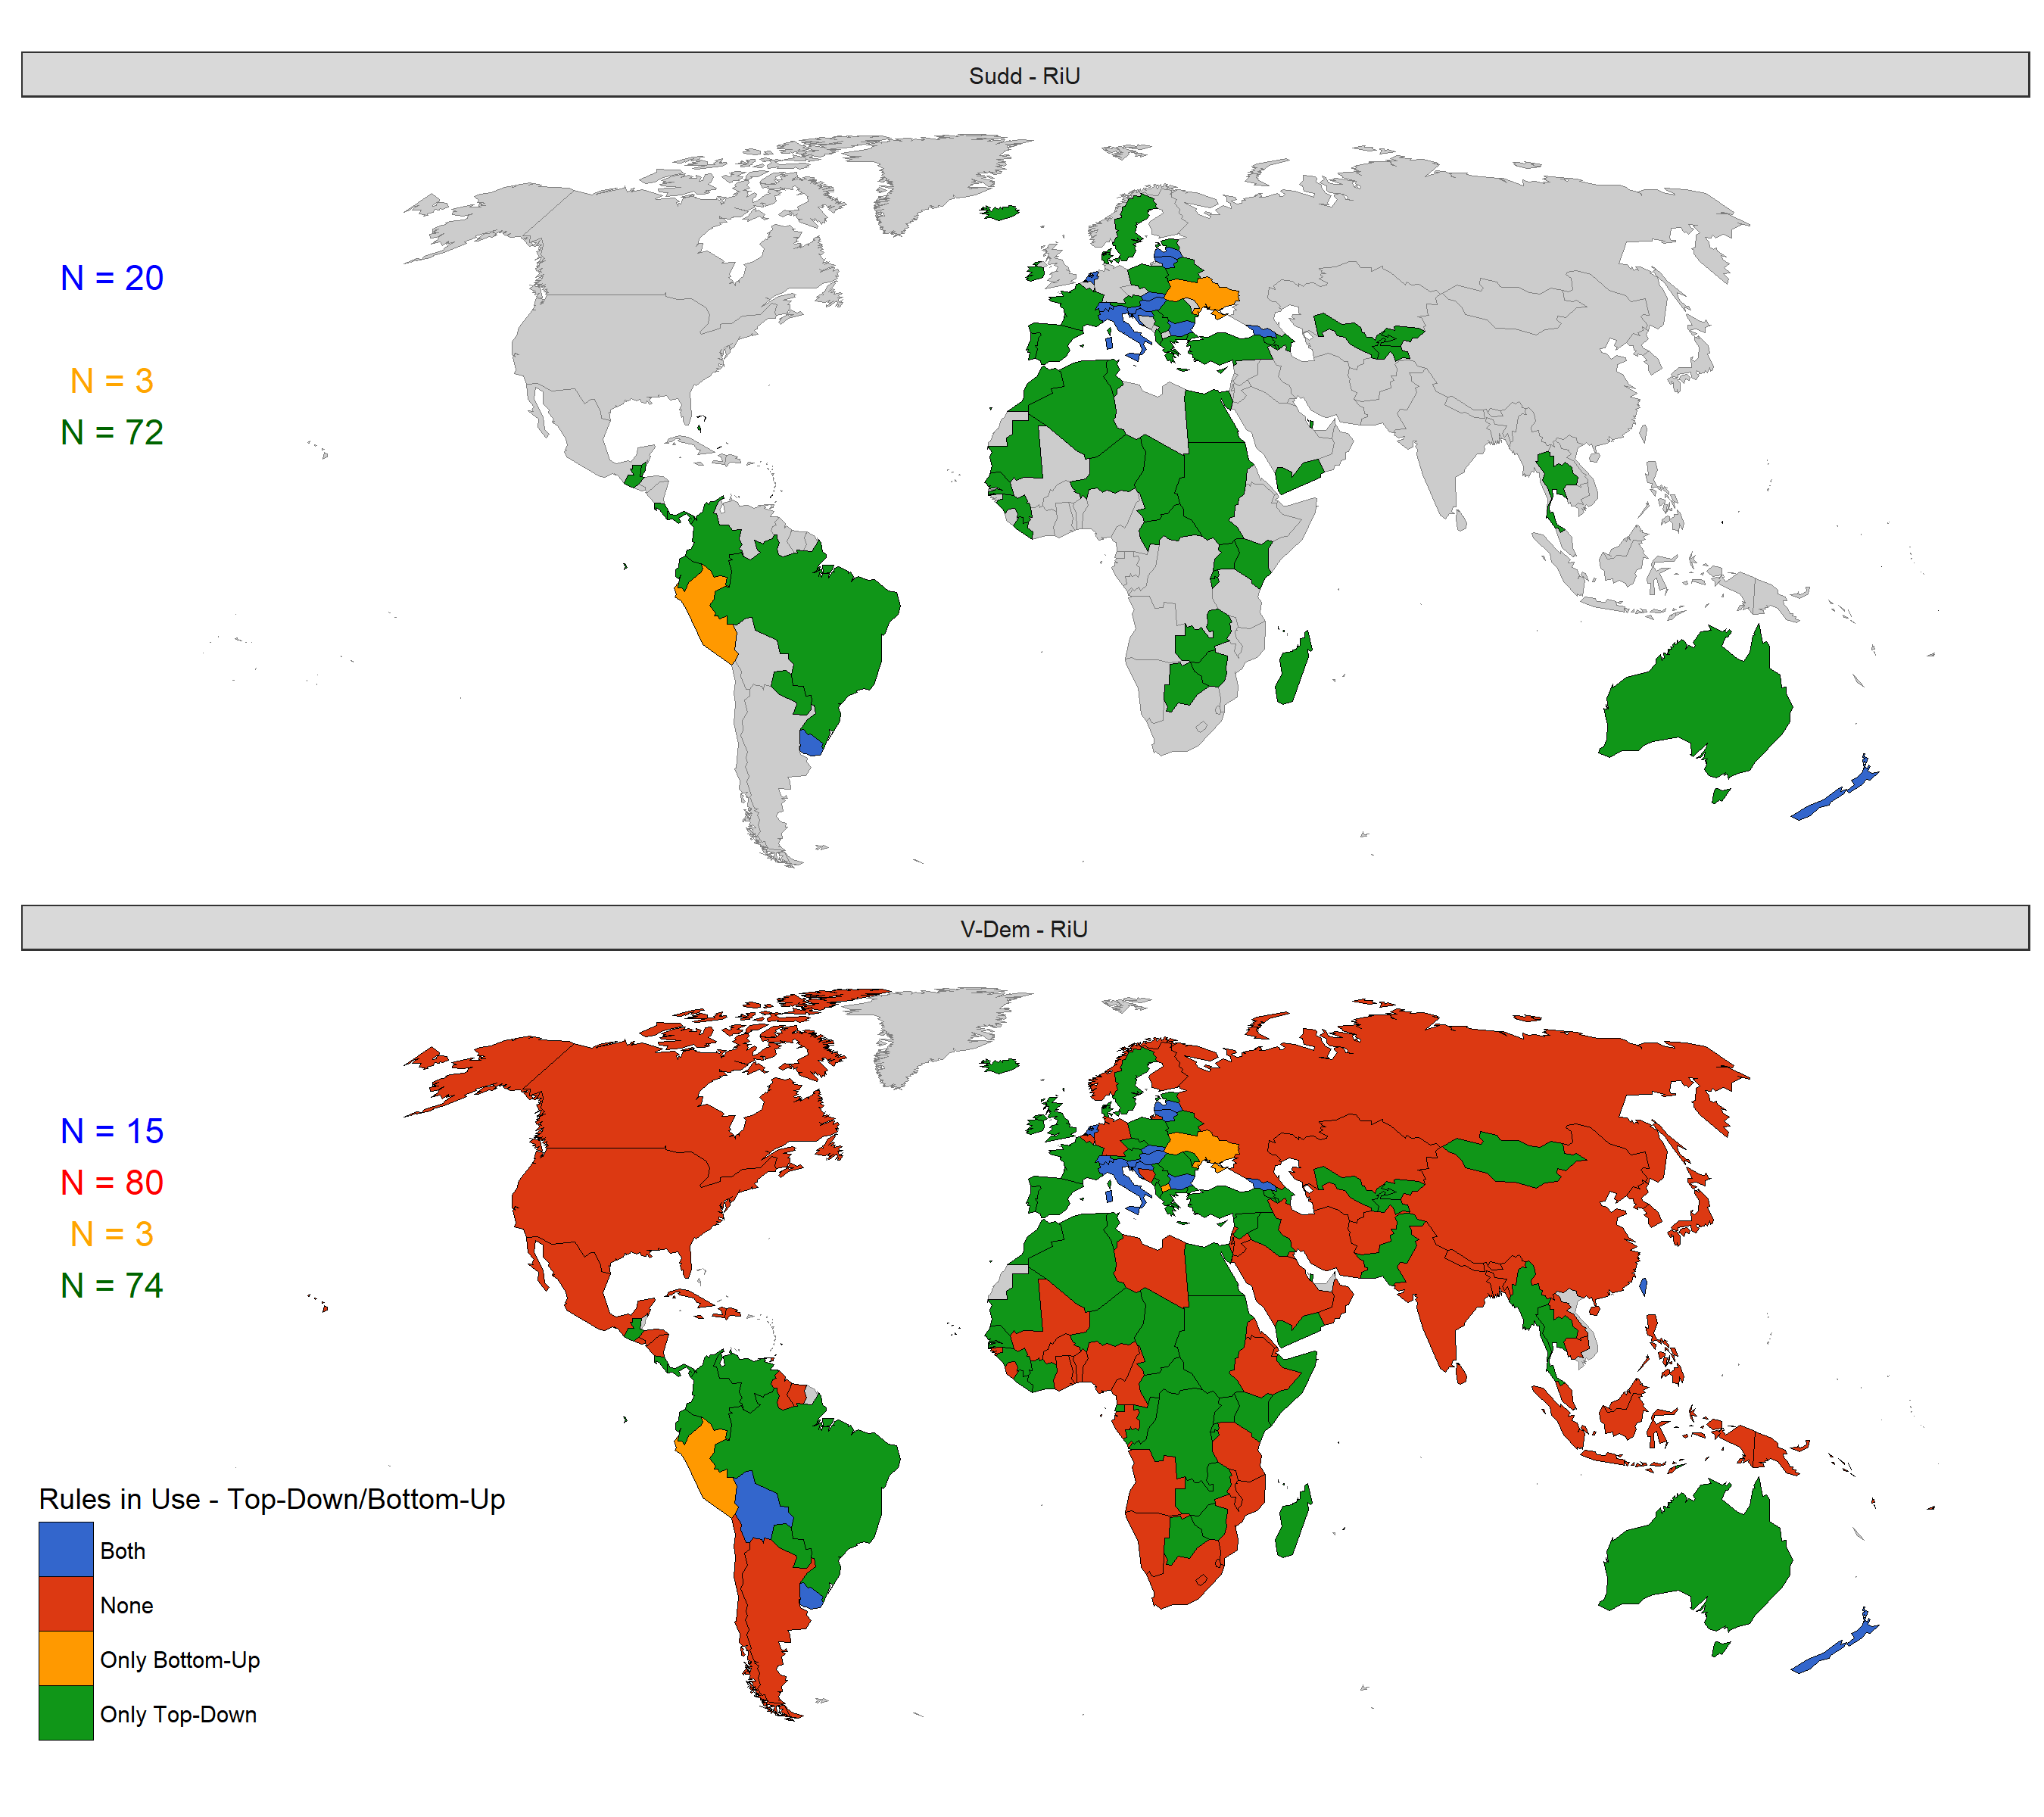
\includegraphics[width=\textwidth]{images/map_riu.png}
	\flushright
	{\scriptsize $^{***}p<0.001$, $^{**}p<0.01$, $^*p<0.05$, $^{\dagger}p<0.1$. Standardized regression coefficients and 90\% confidence intervals are reported. For the full models see Appendix \ref{mod3}. Data weighted to same sample size (=1000). Data Source: see Table \ref{data} in the Appendix. Own calculations  \par}
\end{figure}




\subsection{Comparing Mixed Measures}

 
As we are only assessing two mixed measurement approaches, we compare them in a more detailed way. Figure XX depicts a scatterplot of Fiorinos Direct Democracy Index and the Direct Popular Vote Index from Altman/V-Dem. It becomes visible, that the Fiorino Idex also considers the general level of democracy, while the other measure only accounts for the  direct popular vote dimension. For example, countries like the Ukraine or Venezuela score high on the DPVI, but not on the Direct Democracy Index. In general, there are more countries that get relatively higher scores in the @fiorino2017 measure than the DPVI, for example the Netherlands, Philippines or Belgium. As both indices capture a wide range of variables, and the DPVI is aggregated in a complex fashion while the Direct Democracy Index is a qualitative assessment, diverging scores are not very surprising. In regard to the Freedom House classification, countries labeled as free score higher on average on the Direct Democracy Index than countries of the other two Freedom House categories (see Figure XX). As expected, the DPVI shows no such pattern. In contrary, the median is highest for the countries categorized as not free, though it has to be noted that the boxplots only depict results for the sample available for both indices, which means a  proportionally large number of autocracies are not considered.


\begin{figure}
	\caption{Peters RiF compared to other Rules in Form Measures}
	\label{reg2}
	\includegraphics[width=\textwidth]{images/boxplots_final.png}
	\flushright
	{\scriptsize $^{***}p<0.001$, $^{**}p<0.01$, $^*p<0.05$, $^{\dagger}p<0.1$. Standardized regression coefficients and 90\% confidence intervals are reported. For the full models see Appendix \ref{mod3}. Data weighted to same sample size (=1000). Data Source: see Table \ref{data} in the Appendix. Own calculations  \par}
\end{figure}
mixed.

Annotations: N, 

World maps for both the DDI and the DPVI are depicted in Figures XX and XX respectively. The Fiorino measure indicate high levels of direct democracy especially in Europe (and Australia), while the pattern for the DPVI is quite different. Here, only few countries stand out with high values (for example Switzerland, Uruguay, Venezuela), while Central Europe is shaded darker than in the Fiorino map. So, once again, it becomes visible that only the Fiorino index considers the general level of democracy. 

\begin{figure}
	\caption{Peters RiF compared to other Rules in Form Measures}
	\label{reg2}
	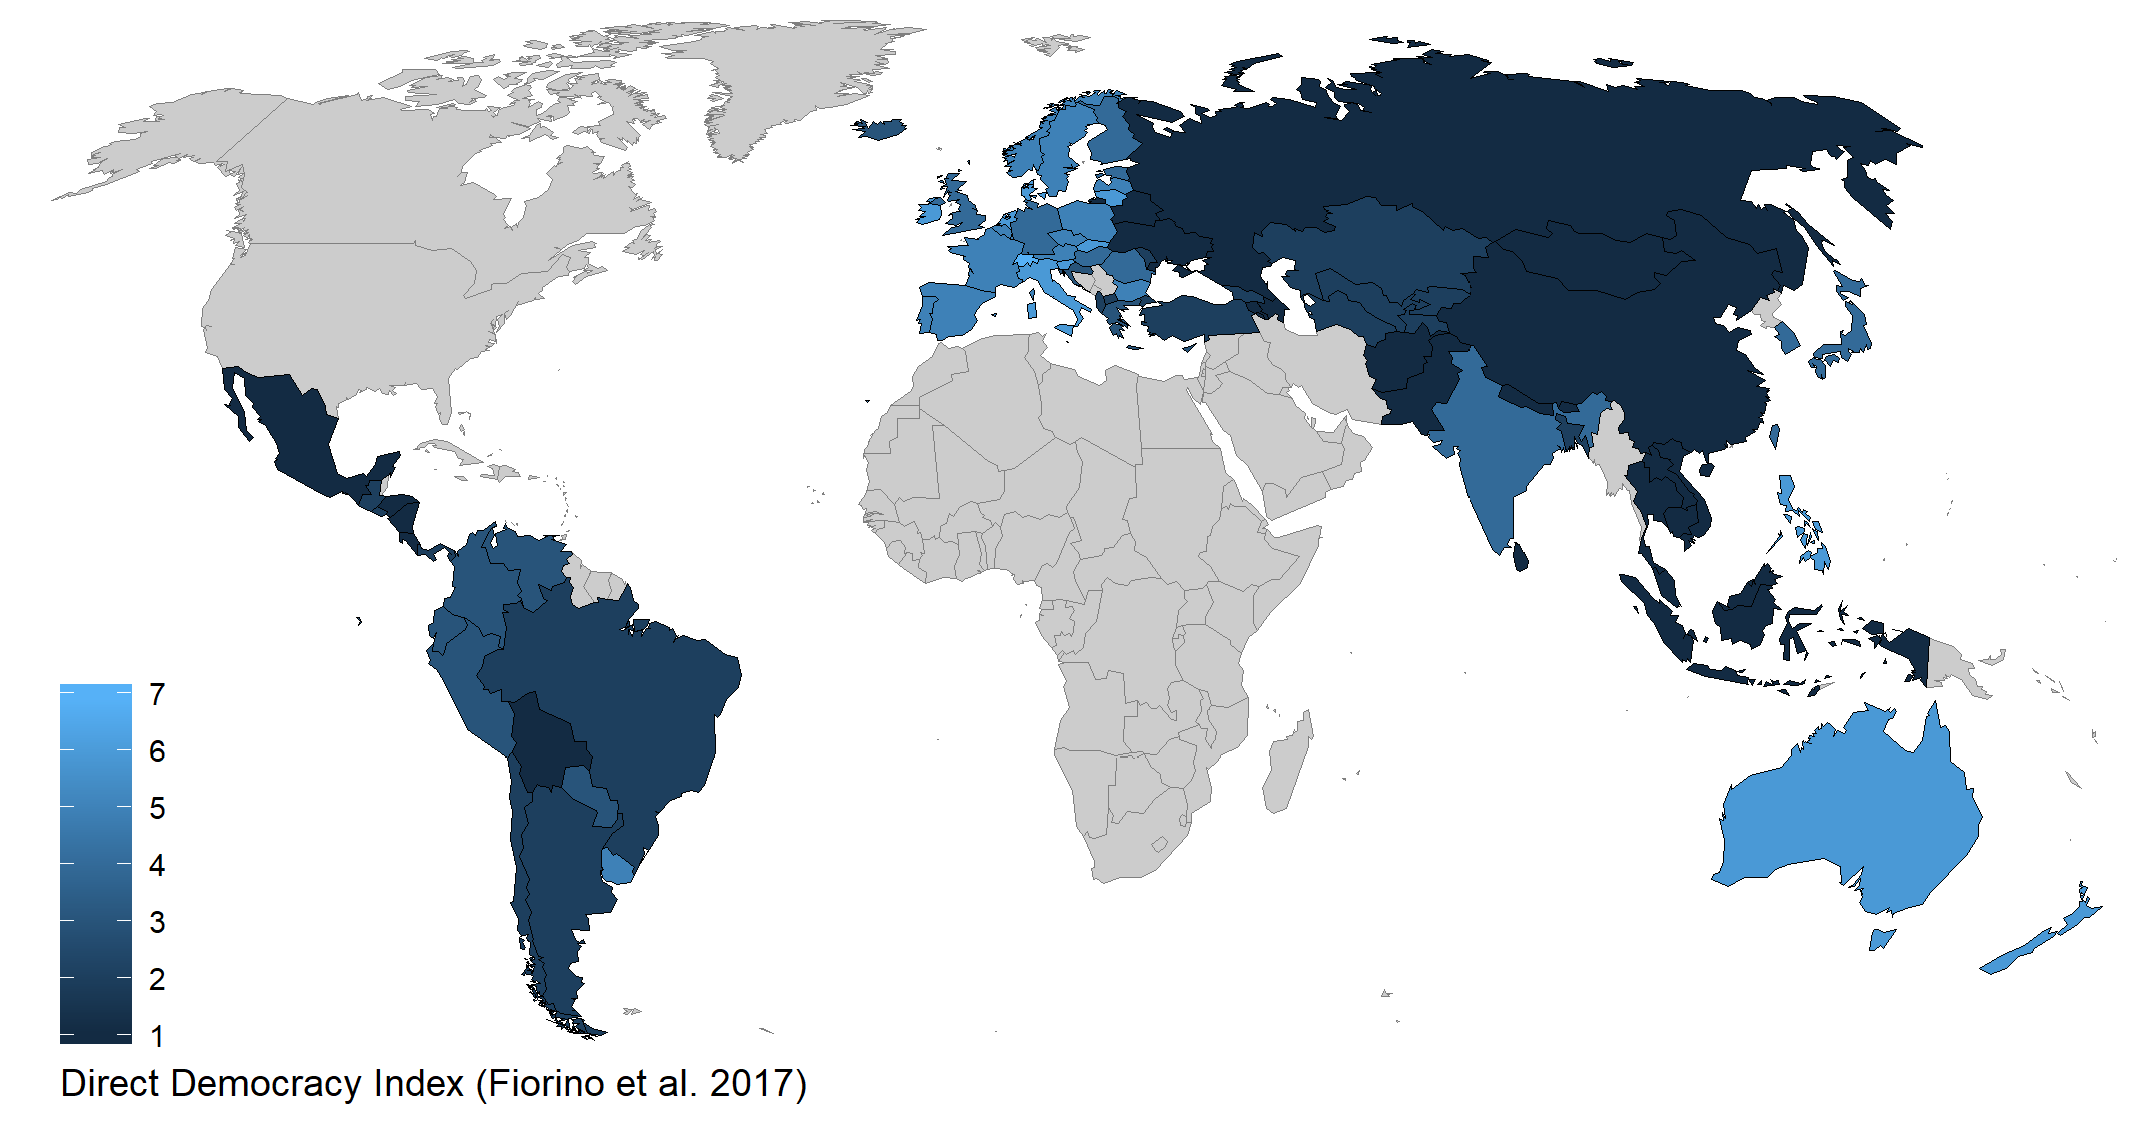
\includegraphics[width=\textwidth]{images/map_fiorini_fin.png}
	\flushright
	{\scriptsize $^{***}p<0.001$, $^{**}p<0.01$, $^*p<0.05$, $^{\dagger}p<0.1$. Standardized regression coefficients and 90\% confidence intervals are reported. For the full models see Appendix \ref{mod3}. Data weighted to same sample size (=1000). Data Source: see Table \ref{data} in the Appendix. Own calculations  \par}
\end{figure}
\begin{figure}
	\caption{Peters RiF compared to other Rules in Form Measures}
	\label{reg2}
	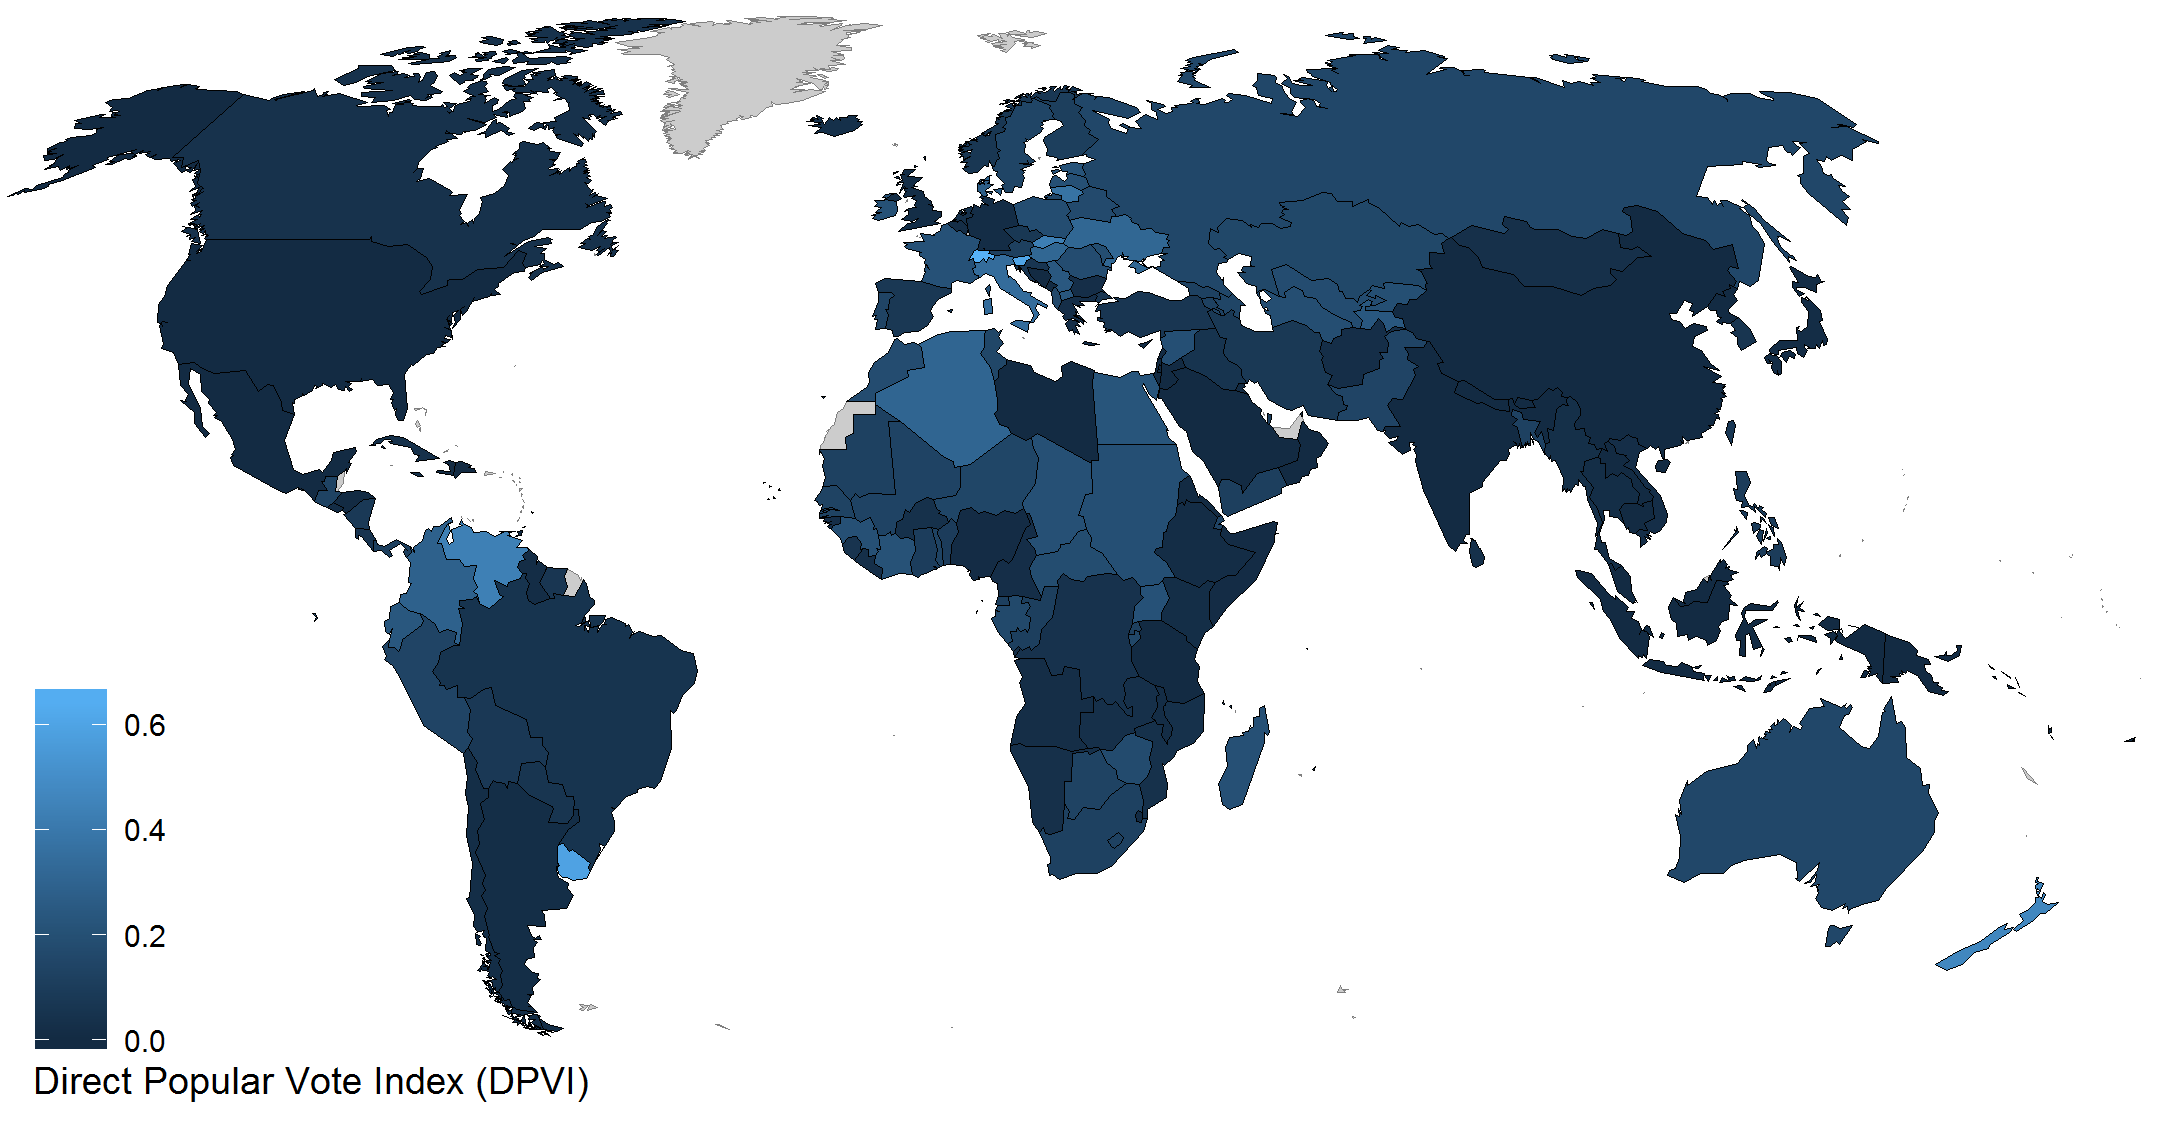
\includegraphics[width=\textwidth]{images/map_altmann_fin.png}
	\flushright
	{\scriptsize $^{***}p<0.001$, $^{**}p<0.01$, $^*p<0.05$, $^{\dagger}p<0.1$. Standardized regression coefficients and 90\% confidence intervals are reported. For the full models see Appendix \ref{mod3}. Data weighted to same sample size (=1000). Data Source: see Table \ref{data} in the Appendix. Own calculations  \par}
\end{figure}



Lastly, we take a look at the DPVI subindices for bottom-up and top-down, as depicted in Figure XX. Countries scoring high primarily on the top-down measure appear in the top-left corner, first and foremost Venezuela, but for example also Algeria, Denmark and Tajikistan. The countries with the highest levels of bottom-up direct popular votes are Slovenia, Switzerland and Uruguay. Comparatively low levels of top-down but high levels of bottom-up direct popular votes can be found for example in Latvia, Georgia and Ukraine. In general, it becomes visible that direct democratic institutions are primarily common in their top-down variant, with only a small number of countries scoring high on the bottom-up sub-index, and most countries having scores of zero. A correlation between the two measures implies an association between top-down and bottom-up indices, however this is mostly based on a few outlier countries that were already discussed (r = 0.24). 


\begin{figure}
	\caption{Peters RiF compared to other Rules in Form Measures}
	\label{reg2}
	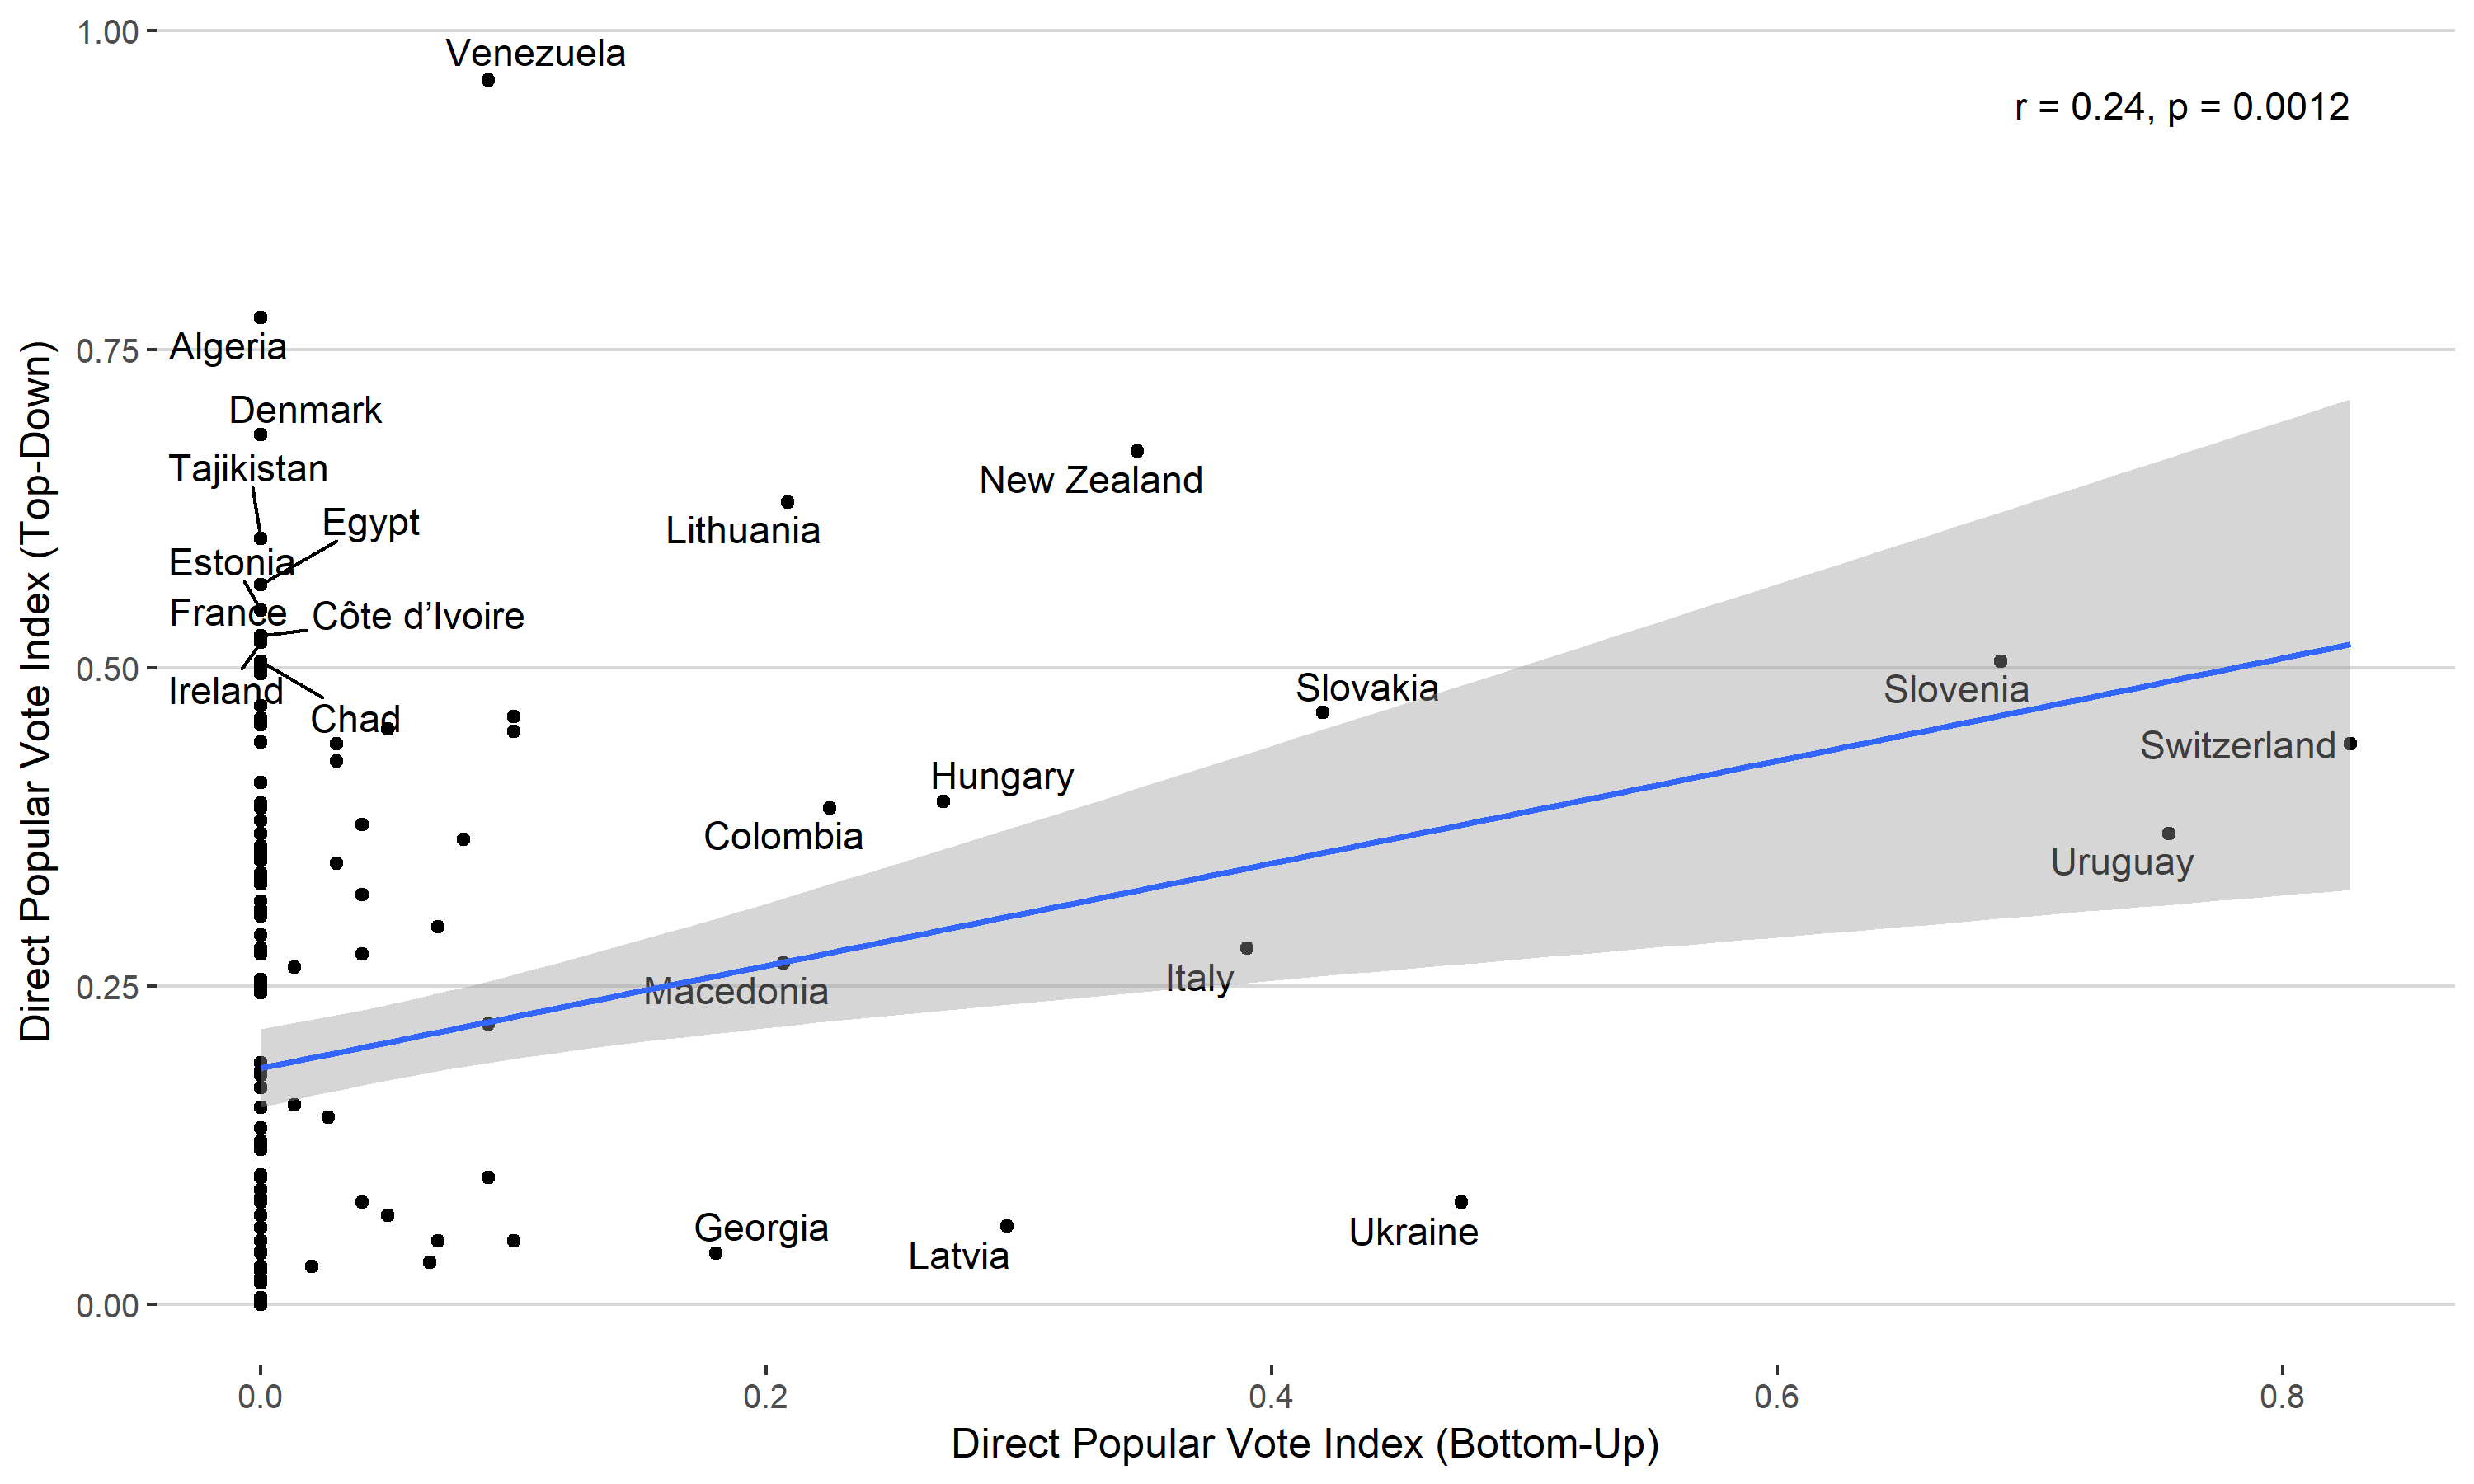
\includegraphics[width=\textwidth]{images/altman_tpbu.png}
	\flushright
	{\scriptsize $^{***}p<0.001$, $^{**}p<0.01$, $^*p<0.05$, $^{\dagger}p<0.1$. Standardized regression coefficients and 90\% confidence intervals are reported. For the full models see Appendix \ref{mod3}. Data weighted to same sample size (=1000). Data Source: see Table \ref{data} in the Appendix. Own calculations  \par}
\end{figure}

%\begin{landscape}
%	\begin{figure}
%		\caption{Democracy Sample: Models A2.1 to F2.2}
%		\label{reg2}
%		\includegraphics[width=730pt,height=430pt]{images/threeway2_fertig.pdf}
%		\flushright
%{\scriptsize $^{***}p<0.001$, $^{**}p<0.01$, $^*p<0.05$, $^{\dagger}p<0.1$. Standardized regression coefficients and 90\% confidence intervals are reported. For the full models see Appendix \ref{mod3}. Data weighted to same sample size (=1000). Data Source: see Table \ref{data} in the Appendix. Own calculations  \par}
%	\end{figure}
%\end{landscape}




%------------------------------- Conclusion --------------------------------%
\section{Conclusion and further Research} \label{conclusion}



Scheint alles noch n bissel willkürlich, wobei es natürlich auch immer auf die Forschungsfrage ankommt….. welche Institutionen man einbezieht, ob diese zB nach td oder bu differenziert werden, ob easiness und decisiveness berücksichtigt werden und wenn ja, wie

subnational democracy und issues are neglected

unified terminology would be great

how to aggregate direct popular vote measures to direct democracy indices?

Limitations of the comparison/study: sometimes a little superficial, due to the scope… for example we could have made a factor analysis

We could have analyized correlations between rules in use and rules in form.. figure in the appendix implies that there isn’t a very strong correlation between them

We could have also analyzed top-down or bottom-up measures per regime type

We found that different direct democracy measures generally overlap substantially with mostly minor differences.. a good sign for the measurement of direct democracy?

In the views of the authors, it is really important for future research to consider a more unified scheme of classifying direct democracy institutions and use, as to ensure comparability and reproducibility between different kinds of research.




%---------------------------------------------------------------------------%
% Bibliography
%---------------------------------------------------------------------------%
\clearpage
\thispagestyle{empty}
%\setstretch{1}
\setstretch{1}
\section{Literature}
\bibliography{references}
%\printbibliography


%---------------------------------------------------------------------------%
% Appendix
%---------------------------------------------------------------------------%
\clearpage
\newpage
\section{Appendix}
\setcounter{table}{0}
\renewcommand{\thetable}{A\arabic{table}}
\renewcommand\thefigure{A\arabic{figure}} 
\setcounter{figure}{0}    
\subsection{Operationalization and Descriptives}

\begin{figure}
	\caption{Peters RiF compared to other Rules in Form Measures}
	\label{reg2}
	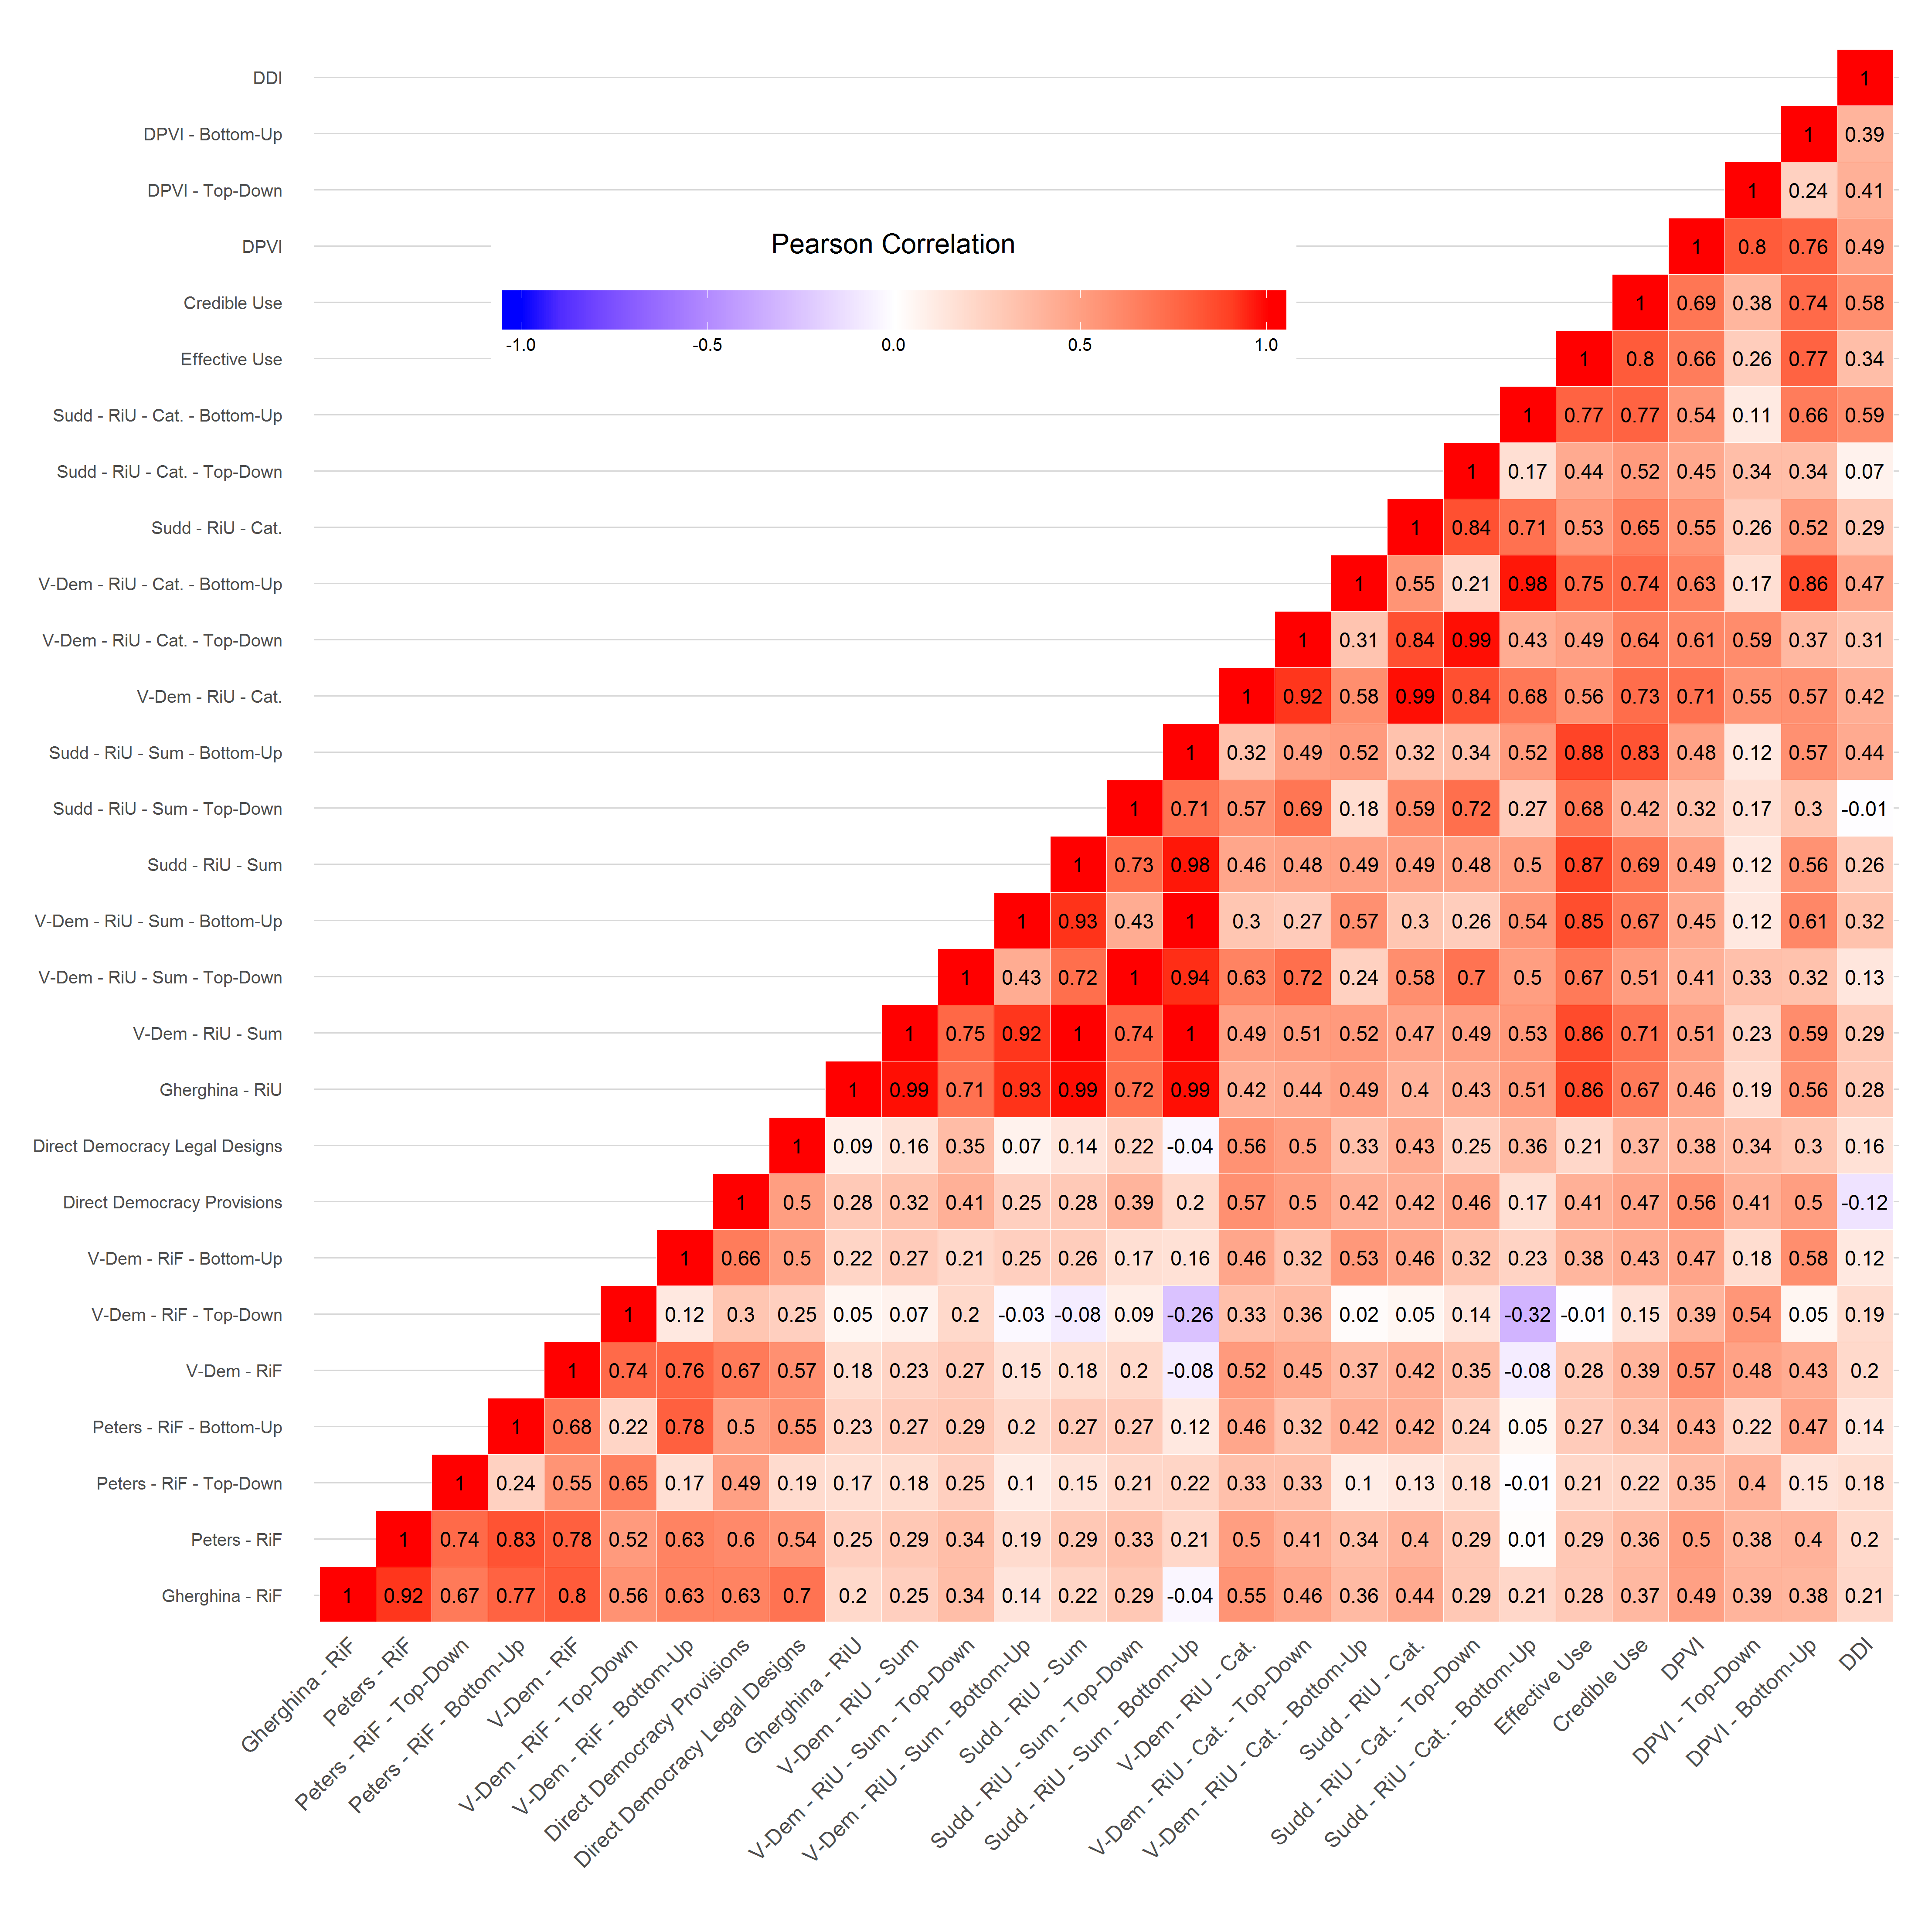
\includegraphics[width=\textwidth]{images/heatmap_fin.png}
	\flushright
	{\scriptsize $^{***}p<0.001$, $^{**}p<0.01$, $^*p<0.05$, $^{\dagger}p<0.1$. Standardized regression coefficients and 90\% confidence intervals are reported. For the full models see Appendix \ref{mod3}. Data weighted to same sample size (=1000). Data Source: see Table \ref{data} in the Appendix. Own calculations  \par}
\end{figure}

\begin{table}[!h]
	\centering
	\caption{Data Sources}
	\label{wuff}
	\begin{tabular}{@{}l@{}}
		\toprule
		\multicolumn{1}{c}{\textbf{Individual-Level Data}} \\ \midrule
		Afrobarometer Round 5/6  \citeyearpar{afro} \\
		AmericasBarometer \citeyearpar{americas} \\
		Asian Barometer Wave 3/4 \citeyearpar{asian} \\
		European Social Survey Round 6 \citeyearpar{european} \\
		Latinobarómetro \citeyearpar{latino} \\
		World Values Survey Wave 6 \citeyearpar{world} \\ \midrule
		\multicolumn{1}{c}{\textbf{Country-Level Data}} \\ \midrule
		Quality of Government - Data \citep{teorell2017qog} \\
		Varieties of Democracy - Data \citep{coppedge2017vdata}
	\end{tabular}
\end{table}
% Please add the following required packages to your document preamble:
% \usepackage{booktabs}


%---------------------------------------------------------------------------%
% Eigenständigkeiterklärung
%---------------------------------------------------------------------------%
\clearpage
\section*{Eigenständigkeitserklärung}
\vspace*{2cm}
\begin{center}
	\begin{minipage}[t]{0.8\textwidth}
		Hiermit versichern wir, dass wir die vorliegende Hausarbeit selbständig und nur mit den angegebenen Hilfsmitteln verfasst haben. Alle Passagen, die wir wörtlich als auch sinngemäß aus der Literatur oder aus anderen Quellen wie z. B. Internetseiten entnommen haben, sind deutlich als Zitat mit Angabe der Quelle kenntlich gemacht.
		
		\vspace*{60mm}
		Stuttgart, 02.10.2017
	\end{minipage}
\end{center}


\end{document}




